%%%%%%%% ICML 2022 EXAMPLE LATEX SUBMISSION FILE %%%%%%%%%%%%%%%%%

\documentclass[nohyperref]{article}

% Recommended, but optional, packages for figures and better typesetting:
\usepackage{microtype}
\usepackage{graphicx}
\usepackage{subfigure}
\usepackage{booktabs} % for professional tables

% hyperref makes hyperlinks in the resulting PDF.
% If your build breaks (sometimes temporarily if a hyperlink spans a page)
% please comment out the following usepackage line and replace
% \usepackage{icml2022} with \usepackage[nohyperref]{icml2022} above.
\usepackage{hyperref}


% Attempt to make hyperref and algorithmic work together better:
\newcommand{\theHalgorithm}{\arabic{algorithm}}

% Use the following line for the initial blind version submitted for review:
\usepackage{icml2022}


\usepackage{bm,amsmath,amsthm,amssymb,multicol,algorithmic,algorithm,enumitem,graphicx}
\usepackage{xcolor}
\usepackage{wrapfig}
\usepackage{url}
\usepackage{multicol}
\usepackage{graphicx}
\usepackage[font=small,skip=0pt]{caption}

\usepackage{xargs}
\usepackage{stmaryrd}
% Recommended, but optional, packages for figures and better typesetting:
\usepackage{microtype}
\usepackage{graphicx}
%\usepackage{subfigure}
\usepackage{booktabs} % for professional tables
\usepackage{mdframed}
\usepackage{multirow}


\theoremstyle{plain}
\newmdtheoremenv{theo}{Theorem}[section]
\newmdtheoremenv{coro}[theo]{Corollary}
\newmdtheoremenv{lem}[theo]{Lemma}

% \newtheorem{theorem}{Theorem}[section]
% \newtheorem{proposition}[theorem]{Proposition}
% \newtheorem{lemma}[theorem]{Lemma}
% \newtheorem{corollary}[theorem]{Corollary}
\theoremstyle{definition}
\newtheorem{definition}[theo]{Definition}
\newtheorem{assumption}[theo]{Assumption}
\theoremstyle{remark}
\newtheorem{remark}[theo]{Remark}

\def\M{\mathcal{M}}
\def\A{\mathcal{A}}
\def\Z{\mathcal{Z}}
\def\S{\mathcal{S}}
\def\D{\mathcal{D}}
\def\R{\mathcal{R}}
\def\P{\mathcal{P}}
\def\K{\mathcal{K}}
\def\E{\mathbb{E}}
\def\F{\mathfrak{F}}
\def\l{\boldsymbol{\ell}}

\newtheorem{Fact}{Fact}
\newtheorem{Lemma}{Lemma}
\newtheorem{Prop}{Proposition}
\newtheorem{Theorem}{Theorem} 
\newtheorem{Def}{Definition}
\newtheorem{Corollary}{Corollary}
\newtheorem{Conjecture}{Conjecture}
\newtheorem{Property}{Property}
\newtheorem{Observation}{Observation}
\newtheorem{Exa}{Example}
\newtheorem{assumption}{H\!\!}
\newtheorem{Remark}{Remark}
\newtheorem*{Lemma*}{Lemma}
\newtheorem*{Theorem*}{Theorem}
\newtheorem*{Corollary*}{Corollary}
 
\newcommand{\eqsp}{\;}
\newcommand{\beq}{\begin{equation}}
\newcommand{\eeq}{\end{equation}}
\newcommand{\eqdef}{\mathrel{\mathop:}=}
\def\EE{\mathbb{E}}
\newcommand{\norm}[1]{\left\Vert #1 \right\Vert}
\newcommand{\pscal}[2]{\left\langle#1\,|\,#2 \right\rangle}
\def\major{\mathsf{M}}
\def\rset{\ensuremath{\mathbb{R}}}

\icmltitlerunning{Layer-wise and Dimension-wise Local Adaptive Method for FL}

\begin{document}

\twocolumn[
% \icmltitle{Layer-wise and Dimension-wise Local Adaptive Method \\
% for Federated Learning}
\icmltitle{Layer-wise and Dimension-wise Adaptive Method for Federated Learning}

% It is OKAY to include author information, even for blind
% submissions: the style file will automatically remove it for you
% unless you've provided the [accepted] option to the icml2021
% package.

% List of affiliations: The first argument should be a (short)
% identifier you will use later to specify author affiliations
% Academic affiliations should list Department, University, City, Region, Country
% Industry affiliations should list Company, City, Region, Country

% You can specify symbols, otherwise they are numbered in order.
% Ideally, you should not use this facility. Affiliations will be numbered
% in order of appearance and this is the preferred way.
\icmlsetsymbol{equal}{*}

\begin{icmlauthorlist}
\icmlauthor{Belhal Karimi}{comp}
\icmlauthor{Xiaoyun Li}{comp}
\icmlauthor{Ping Li}{comp}
\end{icmlauthorlist}

\icmlaffiliation{com}{Cognitive Computing Lab, Baidu Research, 10900 NE 8th St. Bellevue, WA 98004, USA}

\icmlcorrespondingauthor{Belhal Karimi}{belhal.karimi@gmail.com}

% You may provide any keywords that you
% find helpful for describing your paper; these are used to populate
% the "keywords" metadata in the PDF but will not be shown in the document
\icmlkeywords{Adaptive, DNN, Federated, Distributed}

\vskip 0.3in
]

%\printAffiliationsAndNotice{}  % leave blank if no need to mention equal contribution
\printAffiliationsAndNotice{\icmlEqualContribution} % otherwise use the standard text.

\begin{abstract}\vspace{-0.03in}
In the emerging paradigm of Federated Learning (FL), large amount of clients such as mobile devices are used to train possibly high-dimensional models on their respective data. Combining (\textit{dimension-wise}) adaptive gradient methods (e.g. Adam, AMSGrad)
with FL has been an active direction, which is shown to outperform traditional SGD based FL in many cases. In this paper, we focus on the problem of training federated deep neural networks, and propose a novel FL framework which further introduces \emph{layer-wise} adaptivity to the local model updates. Our framework can be applied to many locally adaptive FL methods, including two recent algorithms, Mime~\cite{karimireddy2020mime} and Fed-AMS~\cite{chen2020toward}.
Theoretically, we provide a thorough finite-time convergence analysis of our layer-wise FL methods, coined Fed-LAMB and Mime-LAMB, which matches the convergence rate of state-of-the-art results in FL. Experimental results on various datasets and models, under both iid and non-iid settings,  show that both Fed-LAMB and Mime-LAMB achieve faster convergence speed and better generalization performance, compared to the various recent adaptive FL methods.
\end{abstract}


\section{Introduction}\label{sec:introduction}

A growing and important task while learning models on observed data, is the ability to train over a large number of clients which could either be personal devices or distinct entities.
In the paradigm of Federated Learning (FL)~\citep{konevcny2016federated,mcmahan2017communication}, a central server orchestrates the optimization over those clients under the constraint that the data can neither be gathered nor shared among the clients.
This is computationally more efficient, since more distributed computing resources are used; also, this is a very practical scenario which allows individual data holders (e.g., mobile devices) to train a  model jointly without leaking private data. 
In this paper, we consider the following optimization problem:
\begin{equation}\label{eq:opt}
\min_{\theta} f(\theta) \eqdef \frac{1}{n} \sum_{i=1}^n f_i(\theta)= \frac{1}{n} \sum_{i=1}^n \mathbb E_{\xi\sim \mathcal X_i}[F_i(\theta;\xi)],
\end{equation}
where the nonconvex function (e.g., deep networks) $f_i$ represents the average loss over the local data samples for worker $i \in \inter$, and $\theta \in \mathbb R^d$ the global model parameter. 
$\mathcal X_i$ is the data distribution on each client $i$.
While \eqref{eq:opt} reminds that of standard distributed optimization, the principle and setting of FL are different from the classical distributed paradigm: (i) Local updates: FL allows clients to perform multiple updates on the local models before the global aggregation; (ii) Data heterogeneity: in FL, the local data distributions $\mathcal X_i$ are usually different across the workers, hindering the convergence of the global model. 
FL aims at finding a solution of \eqref{eq:opt} in the fewest number of communication rounds. 


One of the most popular framework for FL is called Fed-SGD~\citep{mcmahan2017communication}: we adopt multiple local Stochastic Gradient Descent (SGD) steps in each device, send those local models to the server that computes the average over the received local model parameters, and broadcasts it back to the devices. Moreover, momentum can be added to local SGD training for faster convergence and better learning performance~\citep{Proc:YuJY_ICML19}. On the other hand, adaptive gradient methods (e.g., Adam~\citep{KB15}, AMSGrad~\cite{reddi2019convergence}) have shown great success in many deep learning tasks. For instance, the update rule of Adam reads as
\begin{equation}\label{rule:adam}
    \begin{aligned}
       \theta_t=\theta_{t-1}-\frac{\alpha m_t}{\sqrt{v_t}},\ \quad &m_t=\beta_1 m_{t-1}+(1-\beta_1) g_t,\\
       & v_t=\beta_2 v_{t-1}+(1-\beta_2) g_t^2,
    \end{aligned}
\end{equation}
where $\alpha$ is the learning rate and $g_t$ is the gradient at time $t$. 
We note that the effective learning rate of Adam is $\alpha/\sqrt{v}$, which is different across dimensions, i.e., \textit{dimension-wise} adaptive. Recently, we have seen growing research efforts in the design of FL frameworks that adopt adaptive gradient methods as the protocols for local model training instead of SGD. 
Examples include federated AMSGrad (Fed-AMS)~\cite{chen2020toward} and Mime~\cite{karimireddy2020mime} with Adam updates. 
Specifically, in both methods, in each round the global server not only aggregates the local models, but also broadcasts to the workers a ``global'' second moment estimation to reconcile the dimension-wise adaptive learning rates across the clients. Therefore, this step can be regarded as a natural mitigation to data heterogeneity, which is a common and important practical scenario that affects the performance of FL algorithms~\citep{li2019federated,liang2019variance,karimireddy2019scaffold}.

In this paper, we focus on improving adaptive FL algorithms. For (single-machine) training of deep neural networks using Adam, \citet{you2019large} proposed a \textit{layer-wise} adjusted learning rate scheme called LAMB, where in each update, the ratio $m_t/\sqrt{v_t}$ is further normalized by the weight of the deep network, respectively for each layer. 
LAMB allows large-batch training which could in particular speed up training large datasets and models like ImageNet~\cite{deng2009imagenet} and BERT~\cite{bert19}. Inspired by the acceleration effect of LAMB, we propose an improved framework for locally adaptive FL algorithms, integrating both \emph{dimension-wise} and \emph{layer-wise} adaptive learning rates in each device's local update. More specifically, \textbf{our contributions} are summarized as follows:

\begin{itemize}
\item We develop Fed-LAMB and Mime-LAMB, two instances of our layer-wise adaptive optimization framework for federated learning, following a principled layer-wise adaptive strategy to accelerate the training of deep neural networks. 


\item We show that our algorithm converges at the rate of $\mathcal{O}\left(\frac{1}{\sqrt{n\tot R}} \right)$ to a stationary point, where $\tot$ is the number of layers of the network, $n$ is the number of clients and $R$ is the number of communication rounds. This matches the convergence rate of LAMB, AMSGrad, as well as the state-of-the-art results in federated learning. The theoretical communication efficiency matches that of Fed-AMS~\cite{chen2020toward}.

\item We empirically compare several recent adaptive FL methods under both homogeneous and heterogeneous data setting on various benchmark datasets. 
Our results confirm the accelerated empirical convergence of Fed-LAMB and Mime-LAMB over the baseline methods, including Fed-AMS and Mime. 
In addition, Fed-LAMB and Mine-LAMB can also reach similar, or better, test accuracy than their corresponding baselines.
\end{itemize}

% \noindent\textbf{Roadmap.} After  a literature review of both realms of federated and adaptive learning in Section~\ref{sec:related}, we develop in Section~\ref{sec:main}, our method, namely Fed-LAMB, based on the computation per layer and per dimension, of the adaptive learning rate in the traditional AMSGrad.
% Theoretical understanding of our method's behaviour with respect to convergence towards a stationary point is developed in Section~\ref{sec:theory} in nonconvex optimization.
% Numerical experiments in Section~\ref{sec:numerical} demonstrate the effectiveness  of our method.


\section{Background and Related Work}\label{sec:related}

Firstly, we summarize some relevant works on adaptive optimization, layer-wise adaptivity and federated learning.


\noindent\textbf{Adaptive gradient methods.}
Adaptive methods have proven to be the spearhead for many nonconvex optimization tasks.
Gradient based optimization algorithms alleviate the possibly high nonconvexity of the objective function by adaptively updating each coordinate of their learning rate using past gradients. 
Common used examples include RMSprop~\citep{TH12}, Adadelta~\citep{Z12}, Adam~\citep{KB15}, Nadam~\citep{dozat2016incorporating} and AMSGrad~\citep{reddi2019convergence}.
Their popularity owes to their great performance in training deep neural networks.
They generally combine the idea of adaptivity from AdaGrad~\citep{DHS11,mcmahan2010adaptive}, as explained above, and the idea of momentum from Nesterov's Method~\citep{N04} or Heavy ball method~\citep{P64} using past gradients.
AdaGrad displays superiority when the gradient is sparse compared to other classical methods~\cite{DHS11}. Yet, when applying AdaGrad to train deep neural networks, it is observed that the learning rate might decay too fast. Consequently,~\citet{KB15} developed Adam whose updating rule is presented in \eqref{rule:adam}. 
A variant, called AMSGrad described in~\citet{reddi2019convergence}, forces $v$ to be monotone to fix the convergence issue. The convergence and generalization of adaptive methods are studied in, e.g.,~\cite{zhou2018convergence,Proc:Chen_ICLR19,zhou2020towards}. 


\noindent\textbf{Layer-wise Adaptivity.} When training deep networks, in many cases the scale of gradients differs a lot across the network layers. When we use the same learning rate for the whole network, the update might be too preservative for some specific layers (with large weights) which may slow down the convergence. Based on this observation, \citet{Proc:LARS18} proposed LARS, an extension of SGD with layer-wise adjusted scaling, whose performance, however, is not consistent accross tasks. Later, \citet{you2019large} proposed LAMB, an analogue layer-wise adaptive variant of Adam. The update rule of LAMB for the $\ell$-th layer of the network can be expressed as
\begin{align*}
    \theta_t^\ell=\theta_{t-1}^\ell-\frac{\alpha \| \theta_{t-1}^\ell\|}{\|\psi_t^\ell\|}\psi_t^\ell,\ \text{with}\ \psi_t^\ell=m_t^\ell/\sqrt{v_t^\ell},
\end{align*}
where $m_t$ and $v_t$ are defined in \eqref{rule:adam}. Intuitively, for the $\ell$-th layer, when the gradient magnitude is too small compared to the scale of the model parameter, we increase the effective learning rate to make the model move sufficiently far. Though the theoretical convergence rate of LAMB is the same as Adam, empirical results in \citet{you2019large} shows that LAMB can significantly accelerate the convergence of Adam in practice, allowing the use of large mini-batch size with much fewer training iterations. 


%\vspace{0.1in}
\noindent\textbf{Federated learning.}
An extension of the well known parameter server framework, where a model is being trained on several servers in a distributed manner, is called federated learning (FL)~\cite{konevcny2016federated,mcmahan2017communication} which has seen many applications in various fields~\cite{Article:YangLCT19,Proc:Leroy_ICASSP19,bonawitz2019towards,Article:NiknamDR20,Proc:XuGSWBW21}. For Fed-SGD (where clients perform SGD-based updates), recent variants and theoretical analysis on the convergence can be found in~\citet{Proc:YuJY_ICML19,karimireddy2019scaffold,Proc:Khaled_AISTATS20,Proc:Li_ICLR20,Proc:Woodworth_ICML20,Proc:WangTBR_ICLR20}.

Recently, several works have considered integrating adaptive gradient methods with FL. \citet{reddi2020adaptive} proposed Adp-Fed where the central server applies Adam-type updates. However, the local clients still perform SGD updates. \citet{chen2020toward,karimireddy2020mime} proposed Fed-AMS and Mime\footnote{``Mime'' in our paper is equivalent to ``MimeLite'' in \cite{karimireddy2020mime}. The original ``Mime'' in \cite{karimireddy2020mime} uses a SVRG-type variance reduction, and has very similar empirical performance as ``MimeLite'' without SVRG.}, respectively, to adopt Adam/AMSGrad at the client level. Both works mitigate the influence of data heterogeneity by ``sharing'' the second moment $v$ (which controls the effective learning rate): in Fed-AMS, a global $v$ is computed and synchronized in each round by averaging the $v_i$'s, $i=1,...,n$ from the local clients; in Mime, a global $v$ is directly calculated using full-batches (averaged over all clients) and maintained at the central server. Hence, Mime requires at least twice computation as Fed-AMS. On many tasks, these methods outperform Fed-SGD and other popular methods like SCAFFOLD~\cite{karimireddy2019scaffold} and FedProx~\cite{Article:Sahu_arxiv18}.



\section{Layer-wise Adaptive Federated Learning}\label{sec:main}

In this section, we introduce our proposed FL framework, admitting both \textit{dimension-wise} adaptivity (of adaptive learning rate) and \textit{layer-wise} adaptivity (of layer-wise scaling). For conciseness, we mainly consider AMSGrad~\cite{reddi2019convergence} as the prototype method. We assume the loss function $f(\cdot)$ is induced by a multi-layer neural network, which includes a broad class of network architectures that can be parameterized layer-by-layer (e.g., MLP, CNN, ResNet, Transformers). Some notations are summarized below.


\noindent\textbf{Notations.} We denote by $\theta$ the vector of parameters taking values in $\rset^p$. 
Suppose the neural network has $\tot$ layers, each with size $p_\ell$ (thus, $p= \sum_{\ell=1}^\tot p_\ell$). For each layer $\ell \in \llbracket \tot \rrbracket$, denote $\theta^\ell$ as the sub-vector corresponding to the $\ell$-th layer. Let $R$ be the number of communication rounds and $T$ be the number of local iterations per round. We denote $\theta_{r,i}^{\ell,t}$ as the model parameter of layer $\ell$ at round $r$, local iteration $t$ and for worker $i$.


% \subsection{Federated Learning with Adaptive Local Updates}

% Firstly, we provide the details of two locally adaptive methods, which serve as the foundation of our approach.

% \noindent\textbf{Fed-AMS~\cite{chen2020toward}.} aa 


% Under the federated learning setting, we stress on the importance of reducing, at each round, the communication cost between the central server, used mainly for aggregation purposes, and the many clients used for gradient computation and local updates.
% Using Periodic Averaging after few local epochs, updating local models on each device, as developed in~\citet{mcmahan2017communication} is the gold standard for achieving such communication cost reduction.
% Intuitively, one rather shifts the computation burden from the many clients to the central server as much as possible. 
% This technique allows for fewer local epochs and a better global model, from a loss minimization (or model fitting) perspective.
% The premises of that new paradigm are SGD updates performed locally on each device then averaged periodically, see~\citet{konevcny2016federated, zhou2017convergence}.
% The heuristic efficiency of local updates using SGD and periodic averaging has been studied in~\citet{stich2018local,Proc:YuJY_ICML19} and shown to reach a similar sublinear convergence rate as in the standard distributed optimization settings.
% Then, with the growing need of training far more complex models, e.g., deep neural networks, several efficient methods, built upon adaptive gradient algorithms, such as Local AMSGrad in~\citet{chen2020toward}, extended both empirically and theoretically the benefits of performing local updates coupled with periodic averaging, especially when dealing with non-iid local data distribution making it a better alternative than local SGD on many learning tasks.



% \subsection{Layer-wise Adaptive Local Update}

\begin{figure}[h]
\mbox{\hspace{-0.15in}
        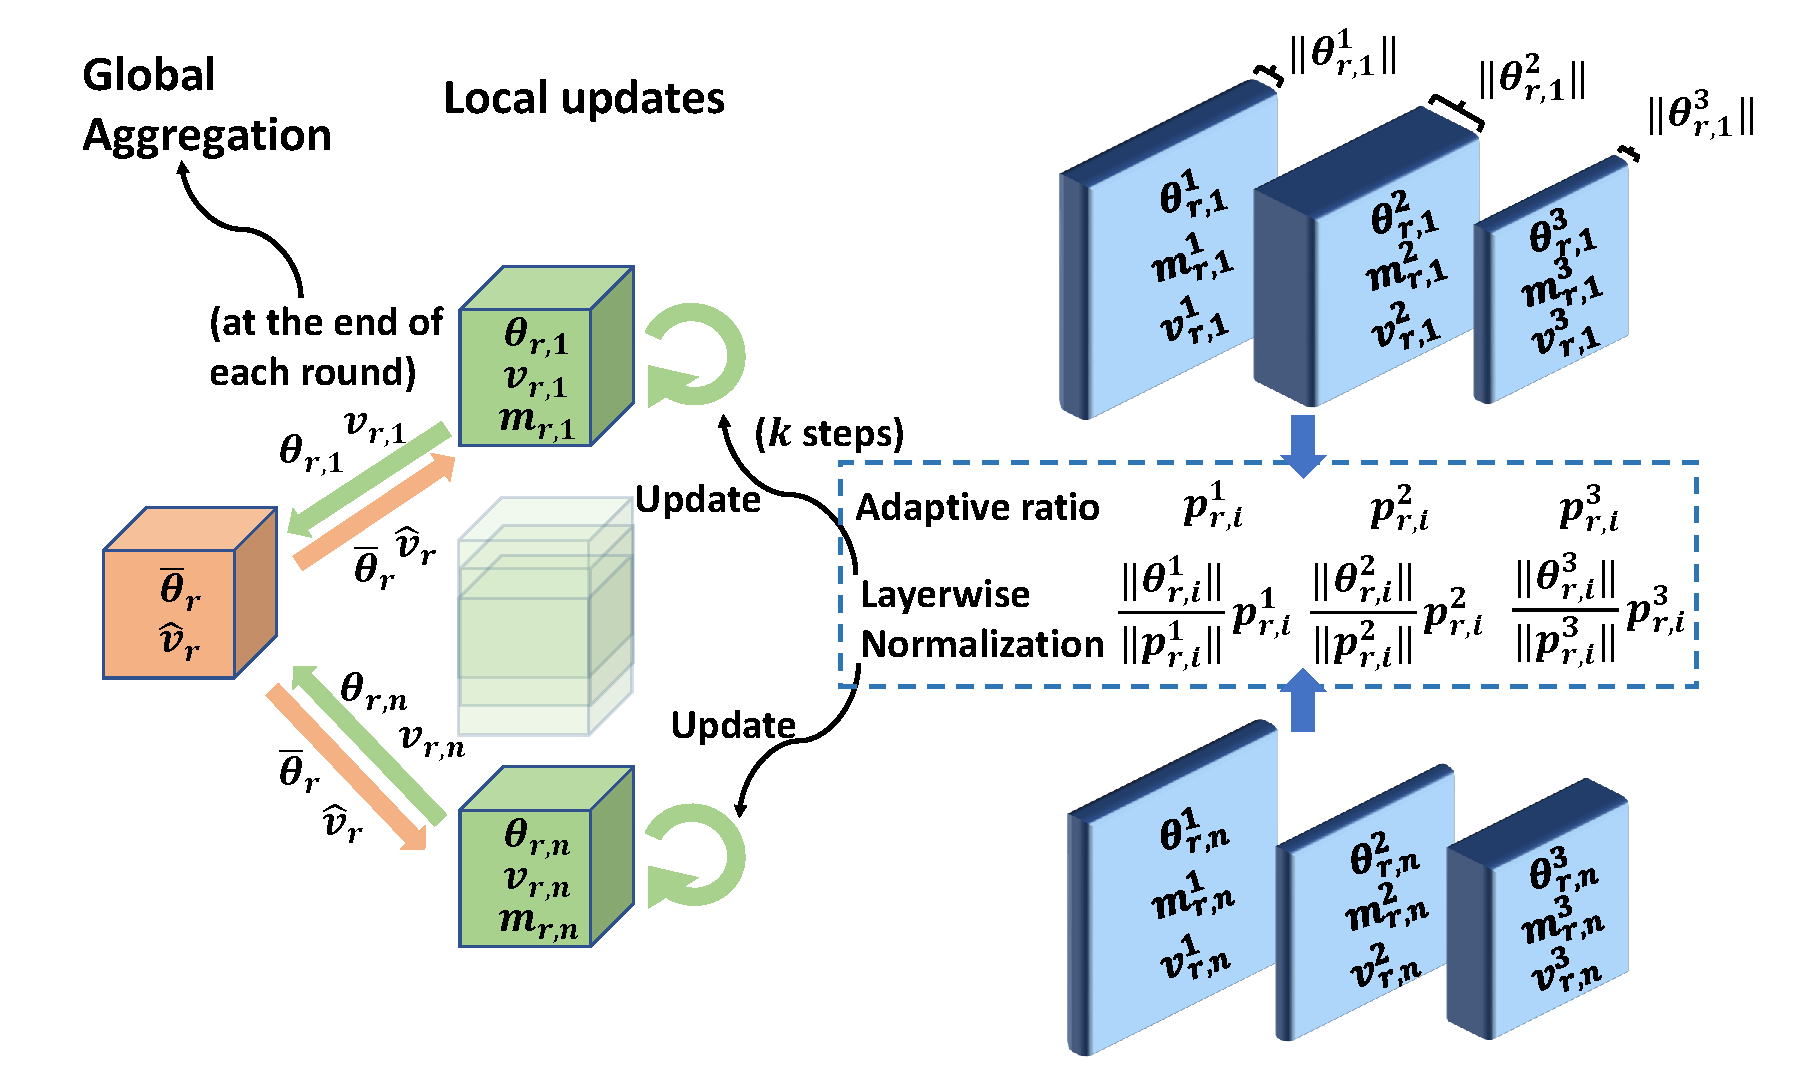
\includegraphics[width=0.53\textwidth]{new_figure/plot1.pdf}
}

	\caption{Illustration of Fed-LAMB framework (Algorithm~\ref{alg:ldams}), with a three-layer network and $\phi(x)=x$ as an example. %	The depth of each network layer represents the norm of its weights. 
		For device $i$ and each local iteration in round $r$, the adaptive ratio of $j$-th layer $\psi_{r,i}^j$ is normalized according to $\Vert \theta_{r,i}^j\Vert$, and then used for updating the local model. 
	At the end of each round $r$, client $i$ sends $\theta_{r,i} =  [\theta_{r,i}^{\ell}]_{\ell =1}^{\tot}$ and $v_{r,i}$ to the central server, which transmits back aggregated $\theta$ and $\hat v$ to devices to complete a round of training.}
	\label{fig:illustrate}
\end{figure}


% \begin{algorithm}[t]
% \caption{ \colorbox{blue!20!white}{Fed-AMS} and \colorbox{green!20!white}{Mime} with LAMB } \label{alg:ldams}
% \begin{algorithmic}[1]
% %\small
% \STATE \textbf{Input}: parameter $0< \beta_1, \beta_2 <1$, and learning rate $\alpha_t$, weight decaying parameter $\lambda \in [0,1]$.
% \STATE \textbf{Initialize}: $\theta_{0,i} \in \Theta \subseteq \mathbb R^d $, $m^0_{0,i}=\hat v^0_{0,i}=v^0_{0,i} = 0$, $\forall i\in \llbracket n\rrbracket$, and $\bar{\theta}_0 =  \frac{1}{n} \sum_{i=1}^n \theta_{0,i}$.
% \FOR{$r=1$ to $R$}
% \FOR{parallel for device $i \in D^{r}$}
% \STATE Set $\theta_{r,i}^{0} = \bar{\theta}_{r-1}$.
% \STATE Set $m^{0}_{r,i} = m^T_{r-1,i}$\ ,\quad $v^{0}_{r,i} = \hat{v}_{r-1}$.
% \FOR{$t=1$ to $T$}
% \STATE Compute stochastic gradient $g^t_{r,i}$ at $\theta_{r,i}^{0}$.
% \STATE $m^t_{r,i} = \beta_1 m^{t-1}_{r,i} + (1 - \beta_1) g^t_{r,i}$ 
% \STATE $m^{t}_{r,i}=m^{t}_{r,i} /\left(1-\beta_{1}^{t}\right)$. \label{line:new1}
% \STATE $v^{t}_{r,i} = \beta_2 v^{t}_{r-1,i} + (1 - \beta_2) (g^t_{r,i})^2$ 
% \STATE $v^{t}_{r,i}=v^{t}_{r,i} /\left(1-\beta_{2}^{t}\right)$. \label{line:new2}
% \STATE Compute the ratio  $\psi_{r,i}^t=m^{t}_{r,i}/(\sqrt{\hat v^{t}_{r}}+\epsilon)$. \label{line:scale}
% \STATE Update local model for each layer $\ell \in \llbracket \tot \rrbracket$: \label{line:layer}
% \begin{equation}\label{eq:updatelayer}
%     \theta_{r,i}^{\ell,t}=\theta_{r,i}^{\ell,t-1}-\frac{\alpha_{r}\phi(\|\theta_{r,i}^{\ell,t-1}\|)(\psi_{r,i}^{\ell,t}+\lambda \theta_{r,i}^{\ell,t-1})}{\|\psi_{r,i}^{\ell,t}+\lambda \theta_{r,i}^{\ell,t-1}\|} \, .
% \end{equation}
% \ENDFOR
% \STATE Devices send $\theta_{r,i}^{T} = [\theta_{r,i}^{\ell,T}]_{\ell =1}^{\tot}$ and $v_{r,i}^T$ to server.
% \ENDFOR
% \STATE Server computes averages of the local models $\bar{\theta}_r = [\bar{\theta}_r^{\ell,T}]_{\ell =1}^{\tot} = [\frac{1}{n} \sum_{i=1}^n \theta_{r,i}^{\ell,T}]_{\ell =1}^{\tot}$ and $\hat{v}_{r+1} = \max( \hat{v}_{r},\frac{1}{n} \sum_{i=1}^n v^T_{r,i} )$ and send them back to the devices. \label{line:final}
% \ENDFOR
% \STATE \textbf{Output}: Global model parameter $\bar{\theta}_R = [\bar{\theta}_R^{\ell,T}]_{\ell =1}^{\tot}$.
% \end{algorithmic}
% \end{algorithm}


\begin{algorithm}[t]
\caption{ \colorbox{blue!20!white}{Fed-LAMB} and \colorbox{green!20!white}{Mime-LAMB} } \label{alg:ldams}
\begin{algorithmic}[1]
%\small
\STATE \textbf{Input}: parameter $0< \beta_1, \beta_2 <1$; learning rate $\alpha$; weight decaying rate $\lambda \in [0,1]$.
\STATE \textbf{Initialize}: $\theta_{0,i} \in \Theta \subseteq \mathbb R^d $; $m^0_{0,i}=\hat v^0_{0,i}=v^0_{0,i} = 0$, $\forall i\in \llbracket n\rrbracket$; $\bar{\theta}_0 =  \frac{1}{n} \sum_{i=1}^n \theta_{0,i}$; $\hat v_0=\epsilon$

\FOR{$r=1$ to $R$}
\STATE Sample a set of clients $D^r$
\FOR{parallel for device $i \in D^{r}$}
\STATE Set $\theta_{r,i}^{0} = \bar{\theta}_{r-1}$,\quad $m^{0}_{r,i} = m^T_{r-1,i}$\ ,\quad $v^{0}_{r,i} = \hat{v}_{r-1}$
\FOR{$t=1$ to $T$}
\STATE Sample a mini-batch from the local data
\STATE Compute stochastic gradient $g^t_{r,i}$ at $\theta_{r,i}^{t-1}$
\STATE $m^t_{r,i} = \beta_1 m^{t-1}_{r,i} + (1 - \beta_1) g^t_{r,i}$
% \STATE $m^{t}_{r,i}=m^{t}_{r,i} /\left(1-\beta_{1}^{t}\right)$ \label{line:new1}
\STATE \colorbox{blue!20!white}{$v^{t}_{r,i} = \beta_2 v^{t}_{r-1,i} + (1 - \beta_2) (g^t_{r,i})^2$ }
% \STATE $v^{t}_{r,i}=v^{t}_{r,i} /\left(1-\beta_{2}^{t}\right)$ \label{line:new2}
\STATE Compute the ratio  $\psi_{r,i}^t=m^{t}_{r,i}/(\sqrt{\hat v_{r-1}})$. \label{line:scale}

\STATE \label{line:layer} Update local model for each layer $\ell \in \llbracket \tot \rrbracket$: 
\begin{equation}\label{eq:updatelayer}
    \theta_{r,i}^{\ell,t}=\theta_{r,i}^{\ell,t-1}-\frac{\alpha_{r}\phi(\|\theta_{r,i}^{\ell,t-1}\|)(\psi_{r,i}^{\ell,t}+\lambda \theta_{r,i}^{\ell,t-1})}{\|\psi_{r,i}^{\ell,t}+\lambda \theta_{r,i}^{\ell,t-1}\|} 
\end{equation} 
\ENDFOR
\STATE Communicate $\theta_{r,i}^{T} = [\theta_{r,i}^{\ell,T}]_{\ell =1}^{\tot}$ to server

\STATE \colorbox{blue!20!white}{Communicate $v_{r,i}^T$ to server}

\STATE \colorbox{green!20!white}{Communicate $\nabla f_i(\bar\theta_{r-1})$ using full local data}

\ENDFOR
\STATE Server compute $\bar{\theta}_r = \frac{1}{|D^{r}|} \sum_{i \in D^{r}} \theta_{r,i}^{T}$

\STATE \colorbox{blue!20!white}{Server compute $\hat{v}_{r} = \max( \hat{v}_{r-1},\frac{1}{|D^{r}|} \sum_{i \in D^{r}} v^T_{r,i} )$}

\STATE \colorbox{green!20!white}{Compute $\nabla f(\bar \theta_{r-1})=\frac{1}{|D^r|}\sum_{i\in D_r}\nabla f_i(\bar \theta_{r-1})$}

\STATE \colorbox{green!20!white}{Compute $v_r = \beta_2 v_{r-1}+(1-\beta_2)\nabla f(\bar \theta_{r-1})^2)$}

\STATE \colorbox{green!20!white}{Update $\hat v_{r}=\max(\hat v_{r-1},v_r$)}

\ENDFOR
\end{algorithmic}

\end{algorithm}
\vspace{-0.1in}

% For training large deep neural networks, \citet{you2019large} proposed LAMB, an acceleration framework for both SGD and adaptive algorithm that allows large-batch training of BERT in hours. The idea is based on the observation that, during the training of large neural networks, different layers may have very different (absolute) scales, while the magnitude of the gradients in these layers may be similar. Intuitively, this means that in some iterations, the parameter may move a too small step even when the direction (negative gradient) is correct. Therefore, \citet{you2019large} proposed to normalize the gradients in each layer according to the scale of the network layer. Effectively, the algorithm assigns different learning rates to different layers. Empirically, this strategy significantly accelerates the convergence for training large deep models.

In general, our proposed algorithm can be viewed as a ``federated LAMB''. 
Based on the two recent works regarding locally adaptive FL mentioned above, we present the framework by two instances, Fed-LAMB and Mime-LAMB, as summarized in Algorithm~\ref{alg:ldams} and depicted in Figure~\ref{fig:illustrate}. We differentiate the steps of these two methods by blue\colorbox{blue!20!white}{(Fed-LAMB)}and green\colorbox{green!20!white}{(Mime-LAMB)}boxes surrounding the text. Both methods use layer-wise adaptive LAMB for local updates (Line~13). The update rule in \eqref{eq:updatelayer} on local clients can be expressed as
\begin{align*}
    \theta \leftarrow \theta-\alpha\frac{\phi(\|\theta\|)}{\|\psi+\lambda\theta\|}(\psi+\lambda\theta),
\end{align*}
where $\phi(\cdot): \mathbb R_+ \mapsto \mathbb R_+$ is a scaling function (usually chosen to be the identity function in practice) and $\lambda$ is the weight decay rate. The main difference between Fed-LAMB and Mime-LAMB is the way the second moment $\hat v$ is synchronized, i.e., the dimension-wise adaptive learning rate. 
Both methods maintain a global $\hat v$ at the central server:
\begin{itemize}
    \item \colorbox{blue!20!white}{Fed-LAMB (Line 20)}: at the end of each communication round, clients $i$ communicates the local $v_{i}$; the server updates the global $\hat v$ by max operation with the averaged $v$, and sends back the $\hat v$.
    
    \item \colorbox{green!20!white}{Mime-LAMB (Line 21-23)}: in each round $r$, the client computes and transmits the gradient at the global model $\bar\theta_r$ using full local data; the server updates the global $v$ and $\hat v$ in the same manner as AMSGrad. 
\end{itemize}
Conceptually, both approaches aim at alleviating the impact of data heterogeneity by ``globally'' reconciling the adaptive learning rates. However, Mime-LAMB needs to calculate the gradients twice, leading to double the computational cost. Moreover, we should note that \eqref{eq:updatelayer} only uses $\hat v_r$, which is fixed per round, hence for all $T$ local updates. 
We choose this strategy here since it has been shown to perform better than the one allowing $\hat v_r^t$ to change during local model training~\cite{karimireddy2020mime}.

To our knowledge, such two-fold adaptivity (dimension-wise and layer-wise) as in Algorithm~\ref{alg:ldams} has not been considered in federated learning literature before. It turns out that, the significant acceleration of LAMB over Adam in the single-machine setting is also beneficial under the federated learning setting. Next, we will demonstrate the advantages of our scheme, both theoretically and empirically.


\vspace{-0.1in}
\section{Convergence Analysis}\label{sec:theory}
%\vspace{-0.05in}

We now present the theoretical analysis for Algorithm~\ref{alg:ldams}.  
Based on classical stochastic nonconvex optimization results, we derive a collection of bounds to understand the convergence behavior of our layer-wise adaptive optimization method under the federated learning framework.
The main challenges we ought to overcome are:
(i) the large amount of decentralized workers working solely on their own data stored locally; 
(ii) a periodic averaging occurs on the central server pushing each of those clients to send local models after some local iterations; 
(iii) both \emph{dimension-wise} and \emph{layer-wise} adaptivity.
Our analysis encompasses those challenges and leads to an informative convergence rates depending on the quantities of interest: the number of layers of the neural network, the number of communications rounds and the number of clients.


\subsection{Finite time analysis of Algorithm~\ref{alg:ldams}}

In the sequel, the analysis of our scheme we provide is \emph{global}, in the sense that it does not depend on the initialization of our algorithm, and \emph{finite-time}, as in it is true for any arbitrary number of communication rounds. In the  context of nonconvex stochastic optimization for federated clients, we need the following common assumptions:
\begin{assumption}\label{ass:smooth}(Smoothness per layer)
For $i \in \inter$ and $\ell \in \llbracket \tot \rrbracket$: $\norm{\nabla f_i (\theta^\ell) - \nabla f_i (\vartheta^\ell)} \leq L_\ell \norm{\theta^\ell-\vartheta^\ell}$.
\end{assumption}
\begin{assumption}\label{ass:boundgrad}(Unbiased and bounded gradient)
The stochastic gradient is unbiased $\forall r,t,i$: $\EE[g_{r,i}^t] = \nabla f_i(\theta_r^t)$ and bounded by $\norm{g_{r,i}^t} \leq M$.
\end{assumption}
\begin{assumption}\label{ass:var}(Bounded variance)
% for any iteration $r>0$, any device $i \in \inter$ and any dimension $j \in \llbracket d \rrbracket$:
The stochastic gradient admits (\emph{locally}) $\EE[|g_{r,i}^j - \nabla f_i(\theta_r)^j|^2] < \sigma^2$, and (\emph{globally}) $ \frac{1}{n} \sum_{i=1}^n ||\nabla f_{i}(\theta_r) - \nabla f(\theta_r)||^2] < G^2$.
\end{assumption}
In particular, Assumption \ref{ass:var} characterizes the data heterogeneity on each device, and $G = 0$ when local data are i.i.d. Also, following~\citet{you2019large}, we use the following assumption on the scaling function $\phi$.
\begin{assumption}\label{ass:phi}(Bounded scale)
For any $a \in \rset_+$, there exist $\phi_m>0,\phi_M>0$ such that $\phi_m \leq  \phi(a) \leq \phi_M$.
\end{assumption}
We now state our main result regarding the non-asymptotic convergence rate of Fed-LAMB and Mime-LAMB in Algorithm~\ref{alg:ldams}. 
The convergence rate for any round reads: \vspace{0.1in}
\begin{theo}\label{th:multiple update}
Under \textbf{Assumption \ref{ass:smooth}-Assumption \ref{ass:phi}}, consider $\{\overline{\theta_r}\}_{r>0}$ obtained from Algorithm~\ref{alg:ldams} with a constant learning rate $\alpha$. Let $\lambda = 0$. Then, for any round $R > 0$,~we~have
\begin{align} \label{bound1multiple}
&  \frac{1}{R}\sum_{r=1}^R  \EE\left[ \left\| \frac{\nabla f(\overline{\theta_r})}{\hat v_r^{1/4}}   \right \|^2 \right] \\\notag
&\leq    \sqrt{\frac{M^2 p}{n}}  \frac{ \triangle}{\tot \alpha R}+\frac{4 \alpha^2 \overline{L} M^2 (T-1)^2 \phi_M^2 (1-\beta_2)p}{\sqrt{\epsilon}} \\\notag
&+4\alpha \frac{M^2}{\sqrt{\epsilon}} +      \frac{\phi_M   \sigma^2}{R n} \sqrt{\frac{1 - \beta_2}{M^2 p}  } + 4\alpha \left[ \phi_M^2\sqrt{M^2+p\sigma^2} \right]     \\\notag
& +4  \frac{\alpha^2 \overline{L}}{\sqrt{\epsilon}}  M^2 (T-1)^2 G^2 (1-\beta_2)p +4\alpha \left[\phi_M \frac{\tot \sigma^2}{\sqrt{n}}\right],
\end{align}
where $\triangle=\EE[f(\bar{\theta}_1)]  - \min \limits_{\theta \in \Theta} f(\theta)$ and $\overline{L}=\sum_{\ell=1}^\tot L_\ell$.
\end{theo}


In Theorem~\ref{th:multiple update}, we assume full client participation. Note that the manifestation of $p$ in the rate is because the variance bound is on each dimension in Assumption \ref{ass:var}. This dependency on $p$ can be removed when Assumption \ref{ass:var} is assumed globally, which is also common in optimization literature. Two important Lemmas are required in the proof of the Theorem above (see complete proof of our bound in the Appendix). The first result gives a characterization of the gap between the averaged model, that is computed by the central server in a periodic manner, and each of the local models stored in each client $i \in \inter$. \vspace{0.1in}
\begin{lem}\label{lemma:iterates}
Consider $\{\overline{\theta_r}\}_{r>0}$, the sequence of parameters obtained running Algorithm~\ref{alg:ldams}. Then for $i \in \inter$ and $r > 0$, the gap $\| \overline{\theta_r} - \theta_{r,i} \|^2$ satisfies:
\beq\notag
\| \overline{\theta_r} - \theta_{r,i} \|^2 \leq \alpha_r^2 M^2 \phi_M^2 \frac{(1-\beta_2)p}{\epsilon} \, ,
\eeq
where $\phi_M$ is defined in Assumption \ref{ass:phi}, $p = \sum_{\ell = 1}^\tot p_\ell$.
\end{lem}

The gap is provably bounded by  quantities  such as the total dimension of the multi-layered model $p$, the learning rate and the upper bound of the  gradient that we assumed via Assumption \ref{ass:boundgrad}.
\vspace{0.1in}

\begin{lem}\label{lemma:ratio}
Consider the global model $\{\overline{\theta_r}\}_{r>0}$. Denote $\overline{\nabla}f(\theta_r)=\frac{1}{n}\sum_{i=1}^n \nabla f(\theta_{r,i})$. For $r > 0$:\vspace{-0.2in}


\beq\notag
\left\| \frac{\overline{\nabla}f(\theta_r)}{\sqrt{ v_r}} \right\|^2 \geq \frac{1}{2} \left\| \frac{\nabla f(\overline{\theta_r})}{\sqrt{ v_r}} \right\|^2 - \overline{L} \alpha^2 M^2 \phi_M^2 \frac{(1-\beta_2)p}{\epsilon}\, ,
\eeq
where $M$ is defined in Assumption \ref{ass:boundgrad} and $\phi_M$ is defined in Assumption \ref{ass:phi}.
\end{lem}


Note that the end goal is to characterize how fast the gradient of the averaged/global parameter $\overline{\theta_r}$ goes to zero, but not the averaged local gradient. 
Hence, we use Lemma~\ref{lemma:ratio} to bound the desired suboptimality conditon $\left\| \frac{\nabla f(\overline{\theta_r})}{\sqrt{ v_r}} \right\|$. 
Besides, using a uniform bound on the moment $\|\hat v_r \| \leq M^2$ and by choosing a suitable decreasing learning rate, we have the following simplified statement:
\vspace{0.1in}
\begin{coro}\label{coro:main}
Under the same setting as Theorem~\ref{th:multiple update}, with $\alpha = \mathcal{O}(\frac{1}{ \sqrt{ \tot R}})$, it holds that
\vspace{-0.1in}
\begin{align} \label{coro:rate}
&\frac{1}{R}\sum_{r=1}^R  \EE\left[ \left\| \nabla f(\overline{\theta_r})   \right \|^2 \right] \\
&\leq \mathcal{O}\left( \frac{\sqrt p}{\sqrt{n\tot R}}+\frac{\sqrt\tot \sigma^2 }{\sqrt{nR}}  + \frac{G^2(T-1)^2p}{R\tot}\right). \notag
\end{align}
\end{coro}

% \begin{coro}\label{coro:main}
% Under the same setting as Theorem~\ref{th:multiple update}, choose $\alpha = \mathcal{O}(\frac{1}{ \sqrt{ RT}})$ and assume $\tot \simeq T$, it holds that
% \begin{align} \label{coro:rate}
% &\frac{1}{R}\sum_{r=1}^R  \EE\left[ \left\| \nabla f(\overline{\theta_r})   \right \|^2 \right] \\
% &\leq \mathcal{O}\left( \frac{\sqrt p}{\sqrt{nRT}}+\frac{\sigma^2 }{\sqrt{nRT}}  + \frac{G^2Tp}{R}\right). \notag
% \end{align}
% \end{coro}

The leading two terms display a dependence of the convergence rate of Fed-LAMB on the initialization and the local variance of the stochastic gradients (Assumption \ref{ass:var}). The last term involves the number of local updates $T$ which relates to the communication efficiency, and the global variance $G^2$ characterizing the data heterogeneity. Next, we provide detailed discussion on the comparison of our bound to related prior work.

%We recall that a $\epsilon-$stationary point is defined by the number of communication rounds $R$ such that $\frac{1}{R}\sum_{t=1}^\mathcal{R}  \EE\left[ \left\| \frac{\nabla f(\overline{\theta_t})}{\hat v_t^{1/4}}   \right \|^2 \right] \leq \epsilon$.


%\begin{Theorem}\label{th:main}
%Assume \textbf{Assumption \ref{ass:smooth}-Assumption \ref{ass:phi}}. Consider $\{\overline{\theta_r}\}_{r>0}$, the sequence of parameters obtained via Algorithm~\ref{alg:ldams} with a decreasing lr $\alpha_r$. Then, if $T=1$ and $\lambda = 0$:
%%\beq \label{bound1}
%%\begin{split}
%%  \frac{1}{R}\sum_{r=1}^R  \EE\left[ \left\| \frac{\nabla f(\overline{\theta_r})}{\sqrt{ v_r^t}}   \right \|^2 \right] 
%%   \leq &  \sqrt{\frac{M^2 p}{n}} \frac{ \EE[f(\bar{\theta}_1)]  - \min \limits_{\theta \in \Theta} f(\theta)}{\tot \alpha_r R}+      \frac{\phi_M   \sigma^2}{R n} \sqrt{\frac{1 - \beta_2}{M^2 p}  } \\
%%  +& \alpha_r \phi_M \sigma \tot p \sqrt{n}+ \frac{ \overline{L}\beta_1^2\tot(1-\beta_2)M^2 \phi^2_M n}{2(1-\beta_1)^2 \epsilon}    \\
%% + &\frac{\alpha_r \beta_1}{1-\beta_1}  \sqrt{(1-\beta_2)p} \frac{\tot M^2}{\sqrt{\epsilon}} +\overline{L} \alpha_r^2 M^2 \phi_M^2 \frac{(1-\beta_2)p}{R\epsilon} 
%%   \end{split}
%%\eeq
%\beq \label{bound1}
%\begin{split}
%  \frac{1}{R}\sum_{r=1}^R  \EE\left[ \left\| \frac{\nabla f(\overline{\theta_r})}{\sqrt{ v_r^t}}   \right \|^2 \right] 
%   \leq   \sqrt{\frac{M^2 p}{n}} \frac{ \EE[f(\bar{\theta}_1)]  - f^*}{\tot \alpha_r R} + \frac{\phi_M}{R} \left[ \frac{(1-\beta_2)\overline{L} \alpha_r^2 M^2 \phi_Mp}{\epsilon} +  \frac{ \sigma^2}{n} \sqrt{\frac{1 - \beta_2}{M^2 p}  }    \right]
%   \end{split}
%\eeq
%where $\overline{L} = \sum_{\ell=1}^\tot L_{\ell}$ is the sum of all smoothness constants, $\tot$ is the total number of layers and $f^* \eqdef \min \limits_{\theta \in \Theta} f(\theta)$.
%\end{Theorem}


\subsection{Comparisons}

We dedicate the following paragraph to a discussion on the bound (and implications) derived above in comparison with known results most relevant to our interest in literature.

%\vspace{0.1in}
\noindent\textbf{LAMB bound in~\citet{you2019large}: }
We start our discussion with the comparison of convergence rate of Fed-LAMB with that of LAMB, Theorem 3 in~\citet{you2019large}. In a single-machine setting, the convergence rate of LAMB is $\mathcal O(\sqrt{p}{\sqrt{\tot T}})$ where $T$ is the number of training iterations. Note the convergence rate of Fed-LAMB is different from that of LAMB in the sense that, the convergence criterion is given at the averaged parameters (global model) at the end of each round. In Corollary~\ref{coro:main}, our rate would match LAMB if we take number of local step $T=1$. This also holds true for any fixed $T$ and $R$ sufficiently large. In addition, the $\mathcal O(\frac{1}{\sqrt{nR}})$ rate of Fed-LAMB implies a \textit{linear speedup} effect: the number of iterations to reach a $\delta$-stationary point of Fed-LAMB decreases linearly in $n$, which displays the merit of distributed (federated) learning. 



% (ii) Assuming that the convergence criterion in both Theorems is of similar order (which happens for a large enough number of rounds), the convergence rate of Fed-LAMB displays a similar $\mathcal{O}(1/R)$ behaviour for the initialization term. That said, despite the distributed (federated) setting, our dimension-wise and layer-wise method benefits from the double adaptivity phenomenon explained above and exhibited in LAMB~\citep{you2019large}, under a central server setting.

 
% It is thus natural to consider the evolution of our objective function, precisely its gradient, evaluated at some global model values --as opposed to the outcome of a single step drift in the central server paradigm. Besides, for ease of interpretation, the LHS of~\eqref{bound1multiple} is summed over all rounds instead of a fictive random termination point. A simple calculation would lead to such characterization found in several nonconvex stochastic optimization paper such as~\citet{ghadimi2013stochastic}.

\noindent\textbf{Fed-AMS bound in~\citet{chen2020toward}: }
We now compare our method theoretically with Fed-AMS, the baseline distributed adaptive method developed in~\citet{chen2020toward}. For clarity, we restate their main result (Theorem~\ref{thm:chen}) under our notations.
\vspace{0.1in}
\begin{theo}[\citet{chen2020toward}]  \label{thm:chen}
Under some regularity conditions and similar assumption as ours, with some properly chosen learning rate, when $T\leq \mathcal O(R^{1/3})$, Fed-AMS has convergence rate \vspace{-0.1in}
\beq \label{eqn:chen rate}
\begin{split}
 \frac{1}{R}\sum_{r=1}^R  \EE\left[ \left\| \nabla f(\overline{\theta_r})   \right \|^2 \right]     \leq  \mathcal O( \frac{\sqrt p}{\sqrt{n R}}).
 \end{split}
\eeq
\end{theo}


Firstly, when the number of rounds $R$ is sufficiently large, both rates \eqref{coro:rate} and \eqref{eqn:chen rate} are dominated by $\mathcal O(\frac{\sqrt p}{\sqrt{n R}})$, matching the convergence rate of the standard AMSGrad, e.g.~\cite{Arxiv:Zhou_18}. Secondly, in~\eqref{coro:rate}, the last term containing the number of local updates $T$ is small as long as $T^4\leq \mathcal O(\frac{Rh}{G^2})$. If we further assume $h\simeq T$, then we get the same rate of convergence as Fed-AMS with $T\leq \mathcal{O}(R^{1/3})$ local iterations, identical to the condition of Fed-AMS. Moreover, when $G$ is small (less data heterogeneity), the bound on $T$ would increase, i.e., we can conduct more local updates. This is intuitive, for example, when $G=0$ in the i.i.d. data setting, $T$ can typically be very large. Similar to the single-machine case, although the theoretical convergence rate of Fed-LAMB does not improve Fed-AMS, we will show the impressive empirical acceleration in the empirical study.


\subsection{Extended discussions}

We provide more discussion on the algorithmic and theoretical properties of Algorithm~\ref{alg:ldams}.


\noindent\textbf{Practical Considerations:} Under our analytic setting and conditions mentioned above, we see that the convergence rate of Fed-LAMB matches many popular federated learning methods in non-convex optimization, e.g., Fed-SGD~\cite{mcmahan2017communication}, Mime~\cite{karimireddy2020mime} and Adp-Fed~\cite{reddi2020adaptive}, at $\mathcal O(\frac{1}{\sqrt{nRT}})$. In practice, when trained with same number of rounds and $R$ and local iterations $T$, Mime, Fed-LAMB and Fed-Mime all require communicating two tensors, while Fed-SGD, Adp-Fed only communicate one tensor (the local model parameter). In addition, Mime and Mime-LAMB needs twice computation as other methods, since an extra full local-batch gradient is computed every round. Note that, there are methods aiming at reducing the number of bits transmitted per round through various compression techniques, see for instance~\citet{haddadpour2020fedsketch,ivkin2019communication,li2019privacy}. Those compression techniques are naturally compatible with our scheme to further reduce the communication, but it is not the focus of this paper.


% Yet, contrary to SCAFFOLD, our method only sends bits once per communication round while SCAFFOLD needs to send two vectors, including an additional control variate term  from the clients to the central server. Our result also matches the communication bound of~\citet{reddi2020adaptive} which adapts Adam~\citep{KB15} to the federated setting. The algorithm of~\citet{reddi2020adaptive} performs adaptive updates only at the central server, while SGD is still used for local updates. In addition, the $1/\sqrt n$ term in convergence rate of our method implies a linear speedup  in the number of clients, which also matches the dependency on $n$ of most federated learning methods. 


%\vspace{0.05in}
\noindent\textbf{Data Heterogeneity:} As we mentioned before, dealing with data heterogeneity is an important topic in federated learning. Works have been conducted (e.g.,~\citet{karimireddy2019scaffold,karimireddy2020mime}) on designing specific strategies to alleviate the negative influence of non-i.i.d. data by using techniques like control variate and SVRG. We note that our scheme is, in some sense, naturally capable of balancing the heterogeneity in different local data distributions. 
As mentioned before, this is largely due to the ``moment sharing'' steps in Algorithm~\ref{alg:ldams}), where the adaptive learning rates guided by the second moment estimation are aggregated among clients periodically. The effectiveness of this approach has been validated in literature, for example, \citet{karimireddy2020mime} found that ``moment sharing'' performs very similarly to ``moment sharing + SVRG'' for Mime in terms of practical performance. Applying SVRG-type correction to Fed-LAMB scheme could be an interesting combination, and we leave it as future investigation.



\section{Experiments}\label{sec:numerical}

In this section, we conduct experiments on benchmark datasets with various network architectures to justify the effectiveness of our proposed method in practice. Our main objective is to validate the benefit of dimension-wise adaptive learning rate when integrated with the locally adaptive FL method.
Our method empirically confirms its merit in terms of convergence speed.
Basically, Fed-LAMB and Mime-LAMB reduce the number of rounds and thus the communication cost required to achieve a similar stationary point (or test accuracy) than the baseline methods. 
In many cases, Fed-LAMB brings notable improvement in generalization over baselines.

\noindent\textbf{Methods.} We evaluate the following five FL algorithms, mainly focusing on recent adaptive approaches: 
\begin{enumerate}
    \item Fed-SGD~\citep{mcmahan2017communication}, standard federated averaging with local SGD updates.
    
    \item Adp-Fed (\emph{Adaptive Federated Optimization}, see Appendix~\ref{app:experiment}), the federated adaptive algorithm proposed by~\cite{reddi2020adaptive}. Adp-Fed performs local SGD updates. At each round $r$, the changes in local models, $\triangle_i=w_{r,i}^T-w_{r,i}^0$, $i=1,...,n$, are sent to the central server for an aggregated Adam update. 
    
    \item Fed-AMS~\citep{chen2020toward}, locally adaptive AMSGrad with adaptive learning rate averaging.
    
     \item Mime~\cite{karimireddy2020mime} with AMSGrad, which performs adaptive local updates with central-server-guided global adaptive learning rate.
    
    \item Our proposed Fed-LAMB and Mime-LAMB (Algorithm~\ref{alg:ldams}), layer-wise accelerated local AMSGrad.
\end{enumerate}
For all the adaptive gradient methods, we set the hyper-parameters~$\beta_1=0.9$,~$\beta_2=0.999$ as recommended~\citep{reddi2019convergence}. For the federated learning environment, we use $n=50$ clients with $0.5$ participation rate, i.e., we randomly pick half of the clients to be active for training in each round. 
We set the local mini-batch size as 128. At each round, the training samples are allocated to the active devices, and one local epoch is completed after all the local devices run one pass over their received samples via mini-batch training. 

We tune the initial learning rate $\alpha$ for each algorithm over a fine grid. For Adp-Fed, there are two learning rates involved. We tune the combination of local learning rate (for local SGD) and global learning rate (for global Adam) over a fine grid. The detailed learning rate tuning diagram can be found in Appendix~\ref{app:experiment}. For Fed-LAMB and Mime-LAMB, the weight decay rate $\lambda$ is tuned from $\{0,0.01,0.1\}$, and we use the identity scaling function for $\phi(\cdot)$.
For each run, we report the test accuracy with the best $\alpha$ and $\lambda$. 
The results are averaged over three independent runs, with same initialization for every method.



%\vspace{0.1in}
\noindent\textbf{Datasets and models.} We experiment with four popular benchmark image classification datasets: MNIST~\citep{lecun1998mnist}, Fashion MNIST (FMNIST)~\citep{xiao2017fashion}, CIFAR-10~\citep{krizhevsky2009learning} and TinyImageNet~\citep{deng2009imagenet}. The MNIST dataset contains 60000 training samples and 10000 test samples, from 10 classes of handwritten digits from 0 to 9. The FMNIST dataset has the same sample size and train/test split as MNIST, but the samples are fashion products (e.g., dress, bags) which makes it harder to train than MNIST. The CIFAR-10 dataset has 50000 training images and 10000 test images, from 10 classes. The TinyImageNet is a subset of the ImageNet dataset. It includes 100000 $64\times 64$ images for from 200 classes for training and 10000 for testing. For MNIST, we apply 1) a simple multi-layer perceptron (MLP), which has one hidden layer containing 200 cells; 2) Convolutional Neural Network (CNN), which has two max-pooled convolutional layers followed by a dropout layer and two fully-connected layers with 320 and 50 cells respectively. This CNN is also implemented for FMNIST. 
For CIFAR-10 and TinyImageNet, we use ResNet-18 ~\cite{Proc:He-resnet16}.



%\vspace{-0.07in}
\subsection{Comparison under i.i.d. settings}
%\vspace{-0.02in}

In Figure~\ref{fig:iid}, we report the test accuracy of MLP trained on MNIST, as well as CNN trained on MNIST and FMNIST, where the data is i.i.d. allocated among the clients. We test 1 local epoch and 3 local epochs (more local iterations). In all the figures, we observe a clear advantage of Fed-LAMB over the competing methods in terms of the convergence speed. In particular, we can see that Fed-LAMB is able to achieve the same accuracy with fewest number of communication rounds, thus improving the communication efficiency. For instance, this can be observed as follows: on MNIST + CNN (1 local epoch), Fed-AMS requires 20 rounds to achieves 90\% accuracy, while Fed-LAMB only takes 5 rounds. This implies a 75\% reduction in the communication cost. Moreover, on MNIST, Fed-LAMB also leads to improved generalisation performance, i.e., test accuracy. Note that, the result on MLP to a good extent provides a straightforward illustration on the benefit of layer-wise adaptivity in Fed-LAMB, since compared with Fed-AMS, the only difference is that the learning rate becomes adaptive to the scale of the single hidden layer in Fed-LAMB. We can draw same conclusions with 3 local epochs. Also, similar comparison holds for Mime-LAMB vs. Mime. In general, the Mime-LAMB variant matches the performance of Fed-LAMB closely. 


\begin{figure}[t]

    \begin{center}
        \mbox{
        \hspace{-0.1in}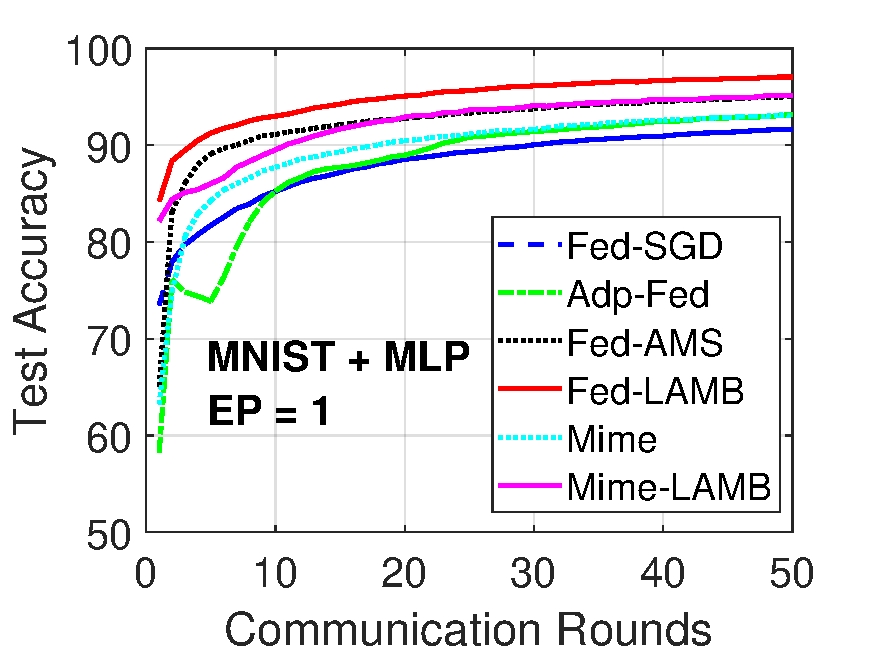
\includegraphics[width=0.26\textwidth]{figure_mime/mnist_testerror_mlp_ep1_iid1_mime.pdf}
        \hspace{-0.1in}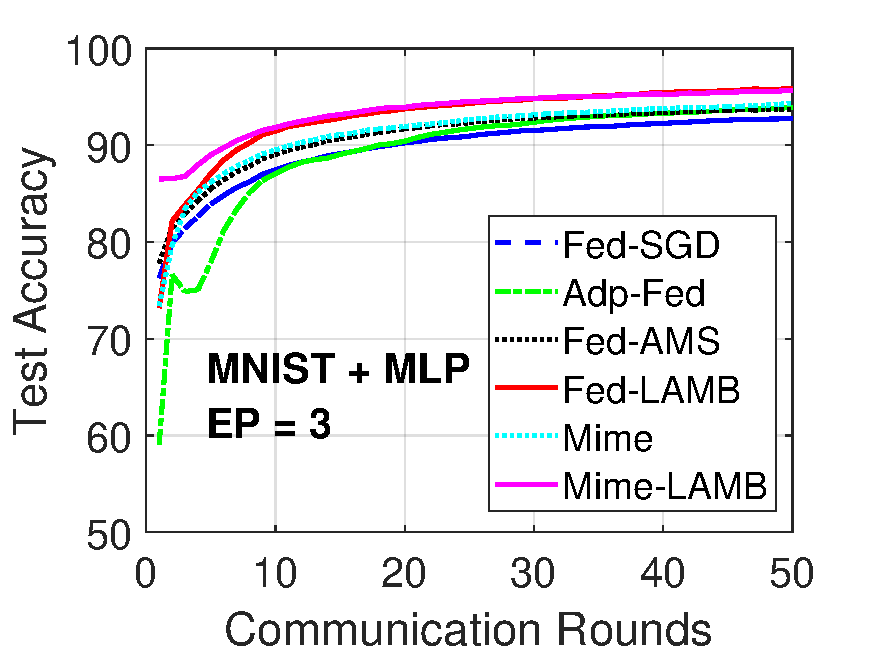
\includegraphics[width=0.26\textwidth]{figure_mime/mnist_testerror_mlp_ep3_iid1_mime.pdf}
                }
        \mbox{
        \hspace{-0.1in}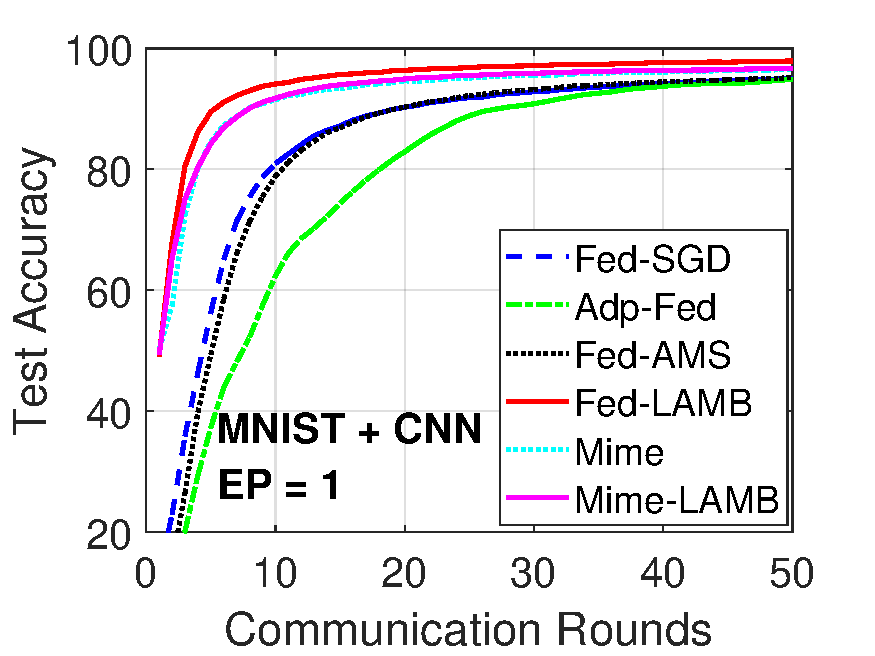
\includegraphics[width=0.26\textwidth]{figure_mime/mnist_testerror_cnn_ep1_iid1_mime.pdf}
        \hspace{-0.1in}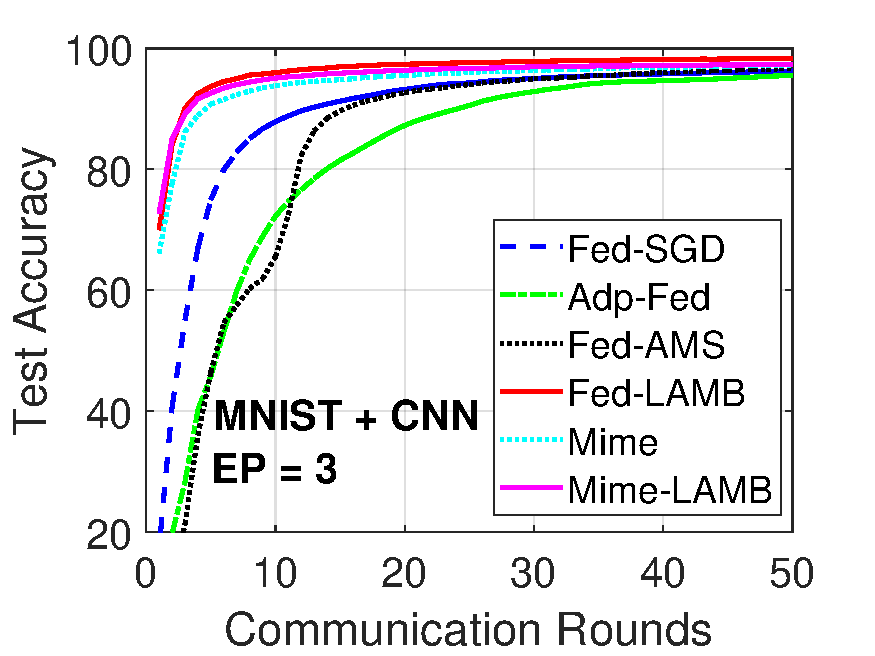
\includegraphics[width=0.26\textwidth]{figure_mime/mnist_testerror_cnn_ep3_iid1_mime.pdf}
                }
        \mbox{
        \hspace{-0.1in}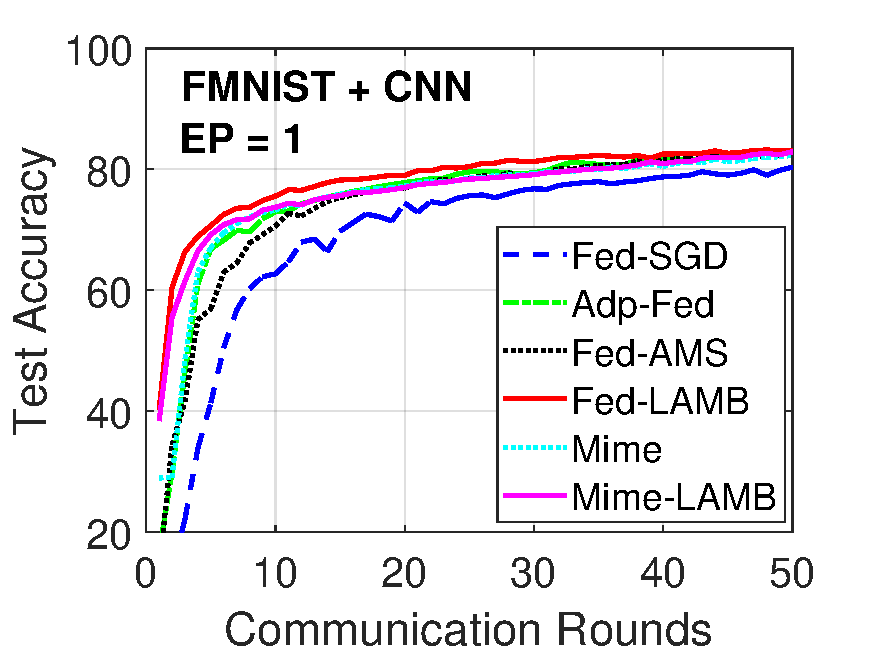
\includegraphics[width=0.26\textwidth]{figure_mime/fmnist_testerror_cnn_ep1_iid1_mime.pdf}
        \hspace{-0.1in}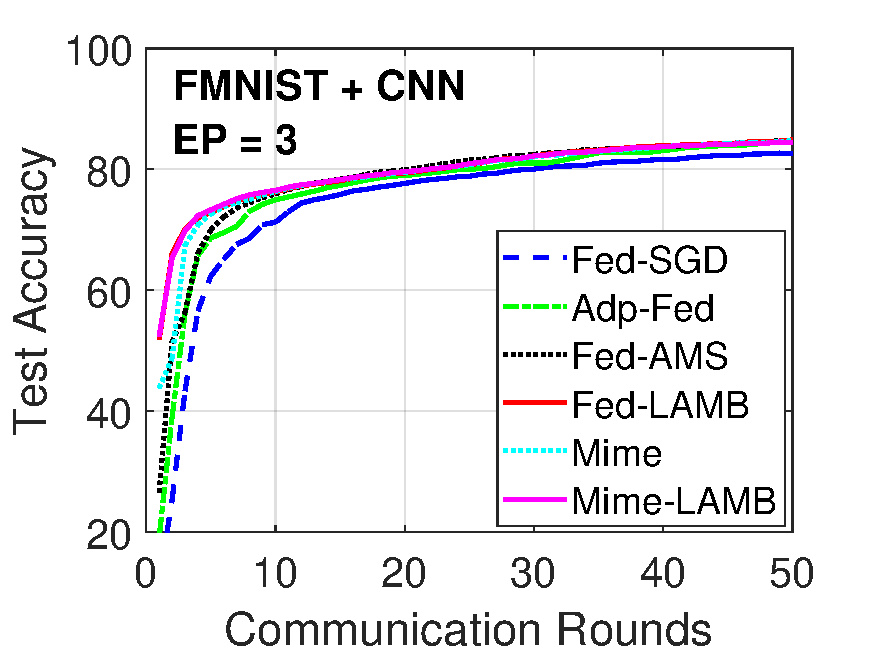
\includegraphics[width=0.26\textwidth]{figure_mime/fmnist_testerror_cnn_ep3_iid1_mime.pdf}
        }
    \end{center}
    \vspace{0.1in}
	\caption{\textbf{i.i.d. data setting}. Test accuracy on MNIST and FMNIST against the number of communication rounds. \textbf{Left Column:} 1 local epoch. \textbf{Right Column:} 3 local epochs. \textbf{1st row:} MNIST + MLP. \textbf{2nd row:} MNIST + CNN. \textbf{3rd row:} FMNIST + CNN. 
	}
	\label{fig:iid}\vspace{-0.2in}
\end{figure}

\begin{figure}[t]

    \vspace{-0.15in}
    \begin{center}
        \mbox{
        \hspace{-0.1in}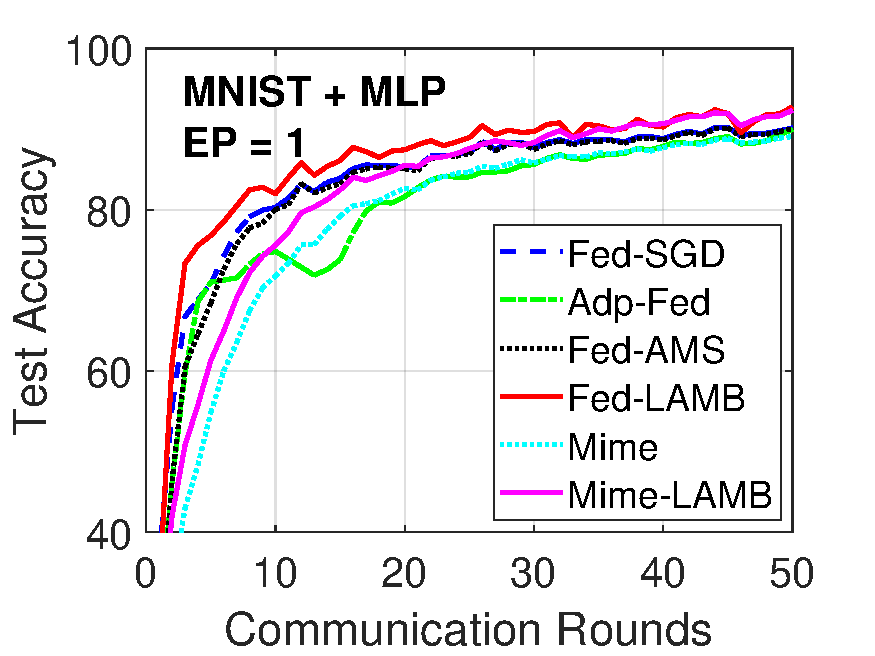
\includegraphics[width=0.26\textwidth]{figure_mime/mnist_testerror_mlp_ep1_iid0_mime.pdf}
        \hspace{-0.1in}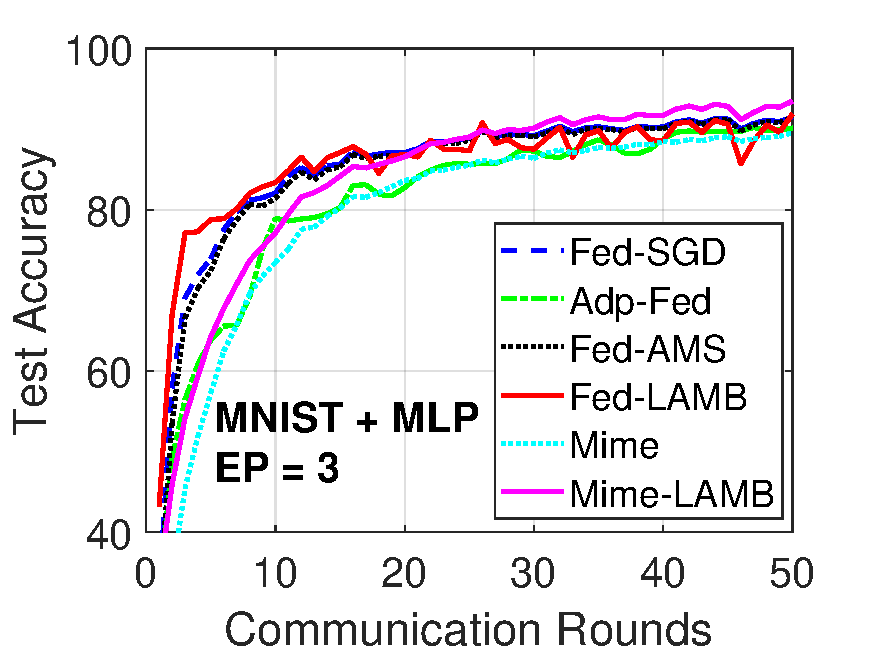
\includegraphics[width=0.26\textwidth]{figure_mime/mnist_testerror_mlp_ep3_iid0_mime.pdf}
                }
        \mbox{
        \hspace{-0.1in}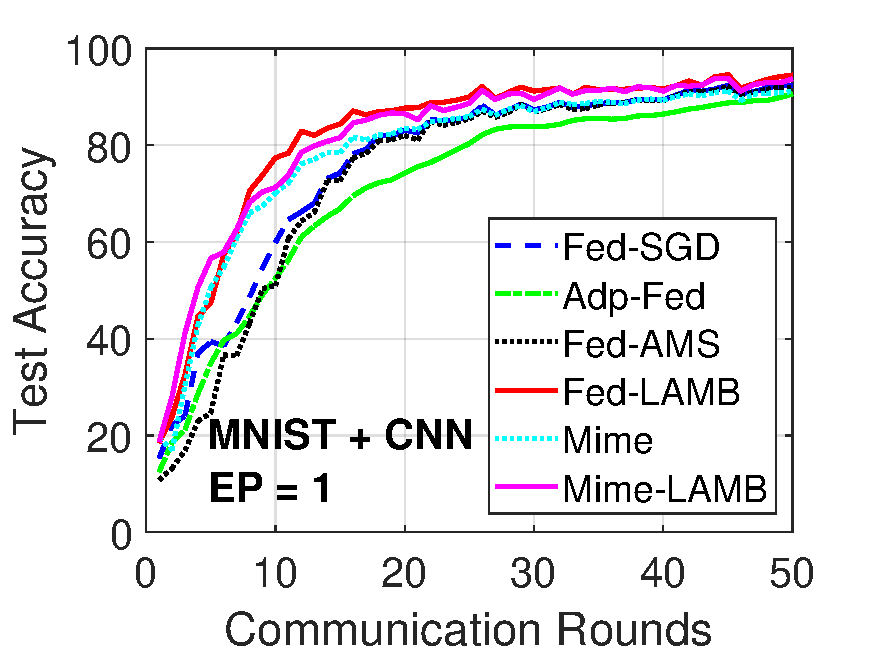
\includegraphics[width=0.26\textwidth]{figure_mime/mnist_testerror_cnn_ep1_iid0_mime.pdf}
        \hspace{-0.1in}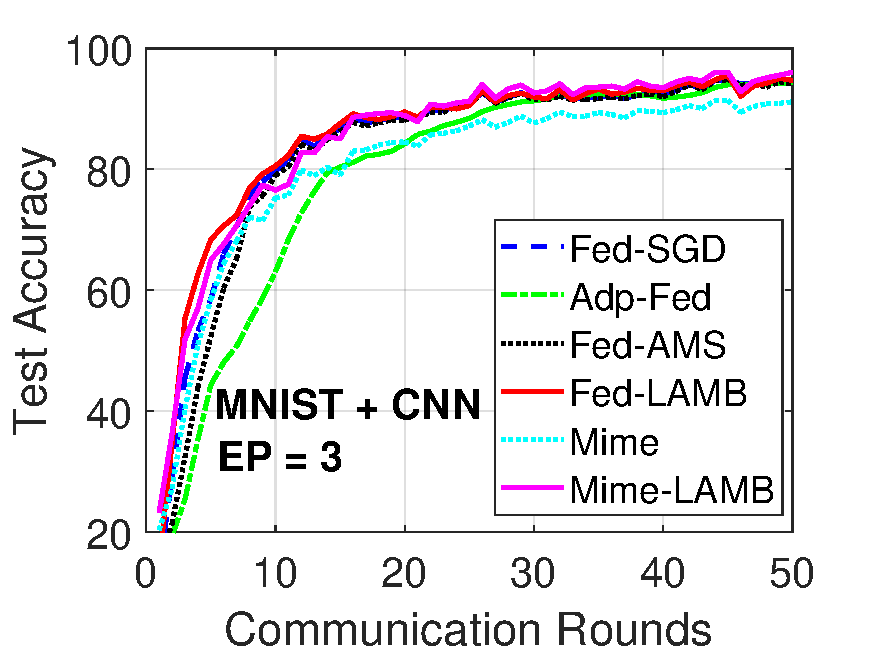
\includegraphics[width=0.26\textwidth]{figure_mime/mnist_testerror_cnn_ep3_iid0_mime.pdf}
                }
        \mbox{
        \hspace{-0.1in}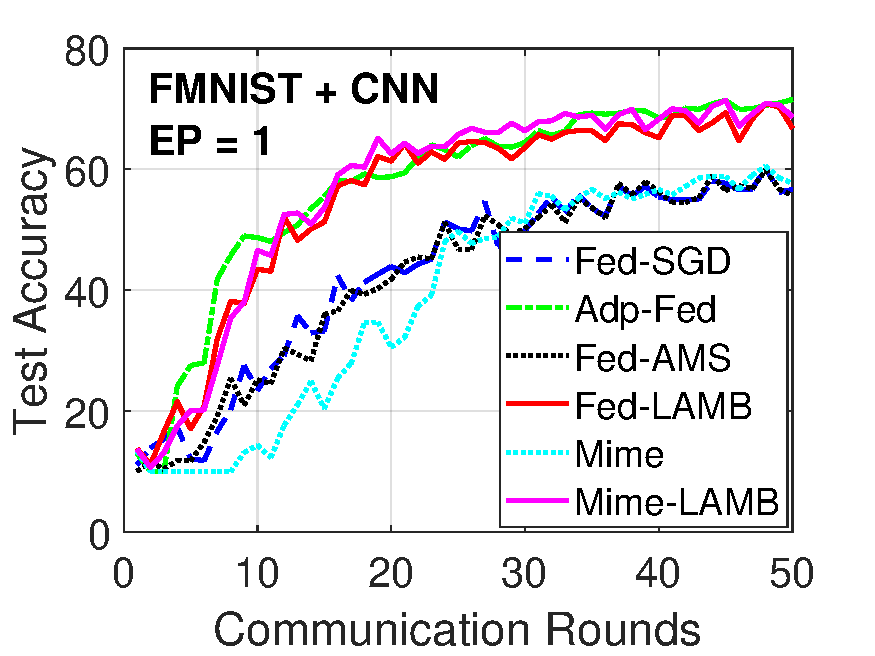
\includegraphics[width=0.26\textwidth]{figure_mime/fmnist_testerror_cnn_ep1_iid0_mime.pdf}
        \hspace{-0.1in}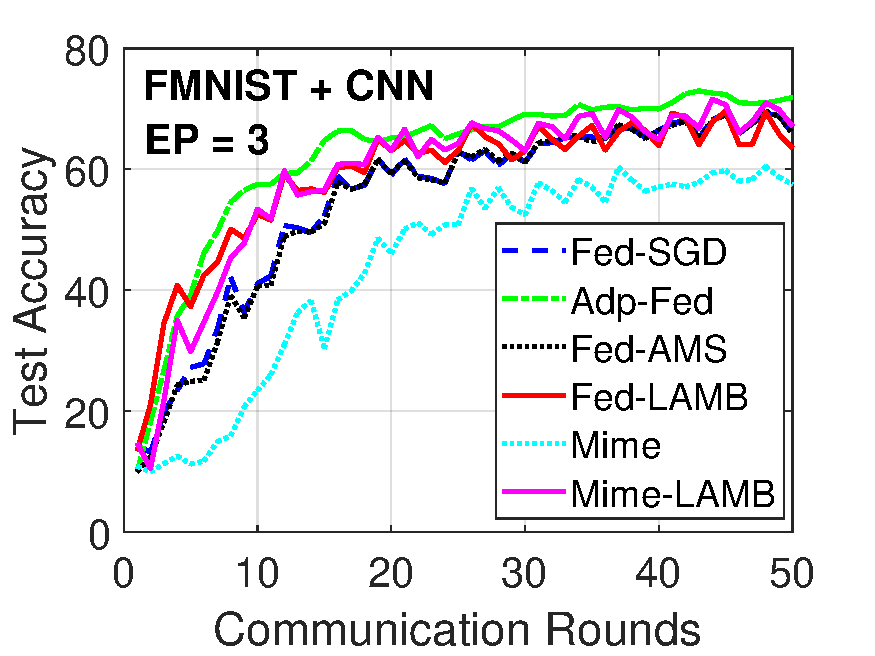
\includegraphics[width=0.26\textwidth]{figure_mime/fmnist_testerror_cnn_ep3_iid0_mime.pdf}
        }
        % \mbox{
        % \hspace{-0.05in}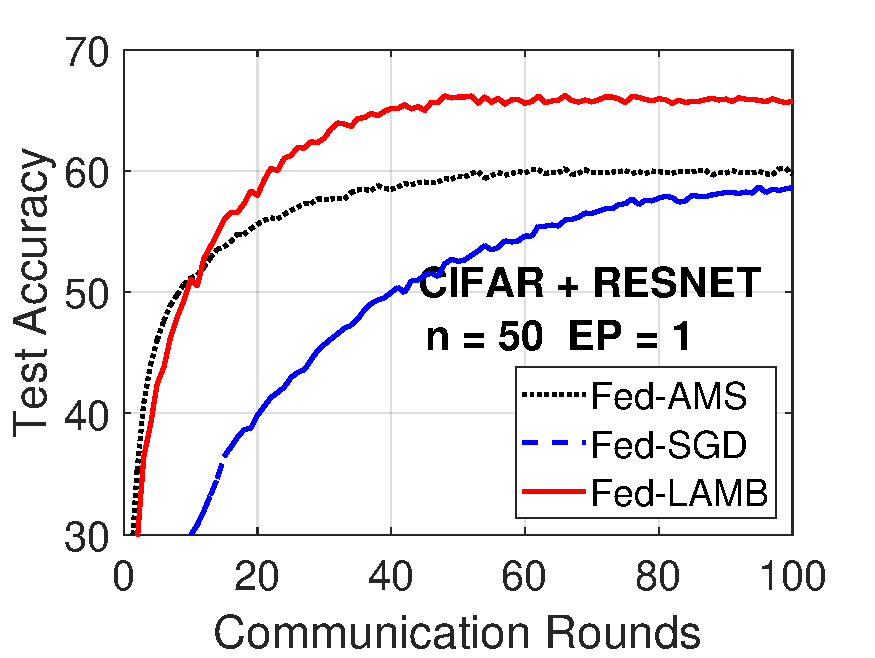
\includegraphics[width=0.26\textwidth]{new_figure/cifar_testerror_resnet_ep1_client50_iid0.pdf}
        % \hspace{-0.1in}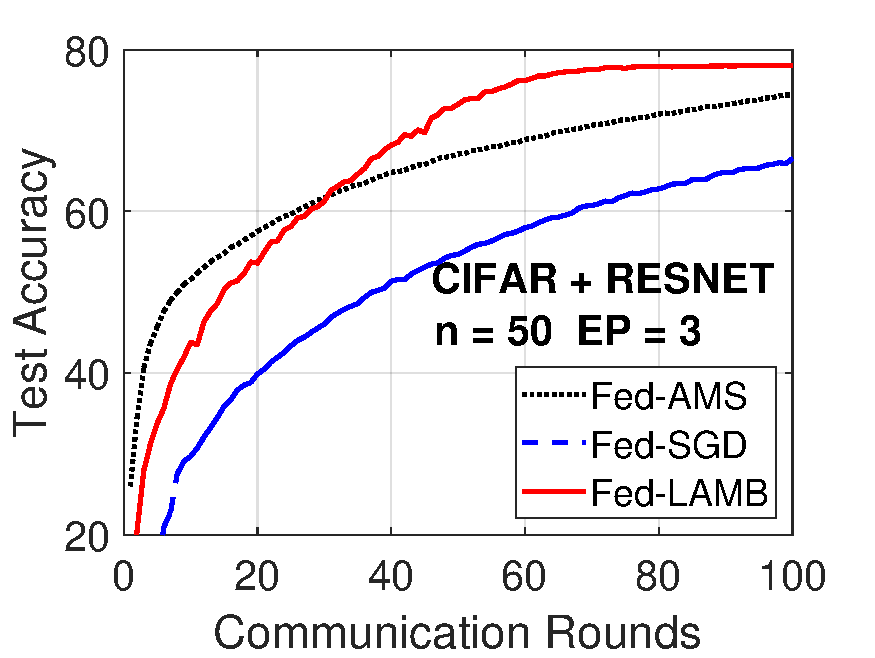
\includegraphics[width=0.26\textwidth]{new_figure/cifar_testerror_resnet_ep3_client50_iid0.pdf}        
        % }
    \end{center}
    \vspace{0.1in}
	\caption{\textbf{non-i.i.d. data setting.} Test accuracy on MNIST and FMNIST against the number of communication rounds. \textbf{Left:} 1 local epoch. \textbf{Right:} 3 local epochs. \textbf{1st row:} MNIST + MLP. \textbf{2nd row:} MNIST + CNN. \textbf{3rd row:} FMNIST + CNN.}
	\label{fig:noniid}	\vspace{-0.1in}
\end{figure}


\begin{table*}[t]
\centering
\caption{Test Accuracy with ResNet-18 Network.}\label{tab:acc}
	\resizebox{2.0\columnwidth}{!}{%
\begin{tabular}{c|cccccc}
\toprule[1pt]
 & Fed-SGD    & Adp-Fed    & Fed-AMS    & \textbf{Fed-LAMB }   & Mime & \textbf{Mime-LAMB}        \\ \hline
CIFAR-10 & 90.75 $\pm$ 0.48  &91.57 $\pm$ 0.38  & 90.93 $\pm$ 0.22 &  \textbf{92.44 $\pm$ 0.53} & 90.94 $\pm$ 0.13 & \textbf{92.00 $\pm$ 0.21}  \\
TinyImageNet & 67.58 $\pm$ 0.21  &  74.17 $\pm$ 0.43   & 64.86 $\pm$ 0.83& \textbf{76.00 $\pm$ 0.26} & 67.82 $\pm$ 0.24 & \textbf{73.46 $\pm$ 0.25} \\
\toprule[1pt]
\end{tabular}
}

\end{table*}




%\vspace{-0.1in}
\subsection{Comparison under non-i.i.d. settings}
%\vspace{-0.02in}




\begin{figure}[h]
\vspace{-0.15in}
    \begin{center}
        \mbox{\hspace{-0.1in}
        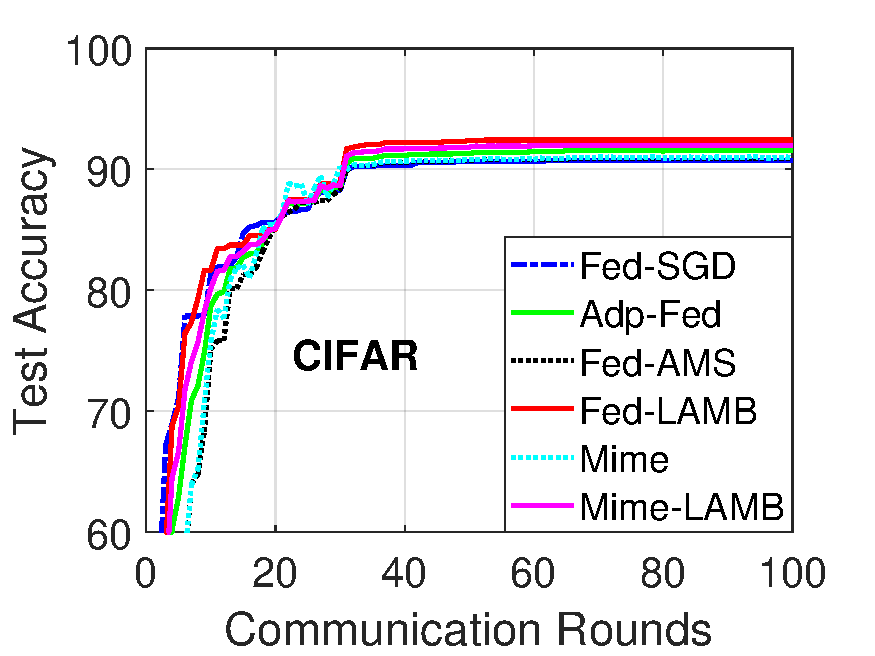
\includegraphics[width=0.26\textwidth]{figure_mime/cifar_testerror_resnet18_ep1_client2_iid0_mime.pdf}
        \hspace{-0.15in}
        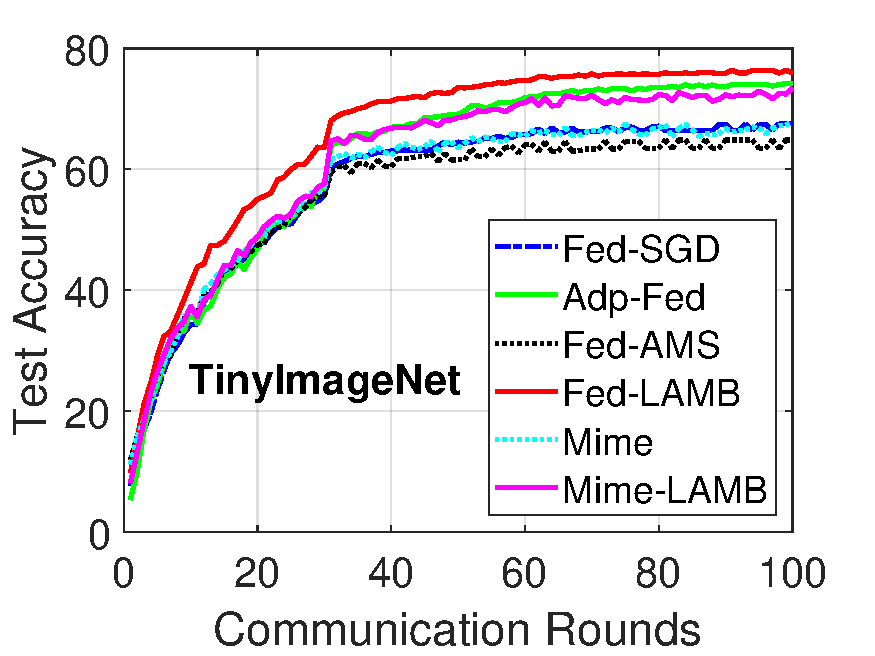
\includegraphics[width=0.26\textwidth]{figure_mime/tinyimagenet_testerror_resnet18_ep1_client2_iid0_mime.pdf}\hspace{-0.1in}
        % \includegraphics[width=0.4\textwidth]{new_figure/tinyimagenet_testerror_resnet18_ep1_client2_iid0.eps}
        }
    \end{center}\vspace{0.1in}
	\caption{\textbf{non-i.i.d. data setting.} Test accuracy on CIFAR-10 + ResNet-18 and TinyImagenet + ResNet-18.
	}
	\label{fig:noniidresnet18}\vspace{-0.1in}
\end{figure}


In Figure~\ref{fig:noniid}, we provide the results on  MNIST and FMNIST, when the local data has non-i.i.d. distribution (i.e., under strong data heterogeneity). In particular, in each round of federated training, every local device only receives samples from one or two class (out of ten). This is known to be the scenario where federated learning is harder to generalize well~\citep{mcmahan2017communication}, thus an important case for the empirical evaluation of FL methods. 
First of all, from Figure~\ref{fig:noniid}, we see that for experiments with 1 local epoch, in all cases our proposed Fed-LAMB outperforms all the baseline methods. Similar to the i.i.d. data setting, Fed-LAMB provides faster convergence speed and achieves higher test accuracy than Fed-SGD and Fed-AMS. The advantage is especially significant for the CNN model, e.g., it improves the accuracy of Fed-SGD and Fed-AMS by more than 10\% on FMNIST. On both two datasets, Fed-LAMB saves around 50\% communication rounds to reach a same accuracy level as Fed-AMS. The other baseline method, Adp-Fed, performs as good as our Fed-LAMB on FMNIST, but worse than other methods on MNIST.

The relative comparison is basically the same when we conduct 3 local epochs. Yet, the advantage of Fed-LAMB becomes less significant than what we observed in Figure~\ref{fig:iid} with iid local data distribution. One plausible reason is that when the local data is highly non-i.i.d., the fast convergence of the local models as in Fed-LAMB might not be as beneficial when we allow too many local iterations. 
Intuitively, learning the local models ``too fast'' might not always be a good thing to the global model, since local models target at different loss functions.
Finally, Mime-LAMB also considerably improves Mime, in all the runs, see Figure~\ref{fig:noniid}.





In Figure~\ref{fig:noniidresnet18}, we present the results on CIFAR-10 and TinyImageNet datasets trained by ResNet-18. When training these two models, we decrease the learning rate to $1/10$ at the 30-th and 70-th communication round. From Figure~\ref{fig:noniidresnet18}, we can draw similar conclusion as before: the proposed Fed-LAMB is the best method in terms of both convergence speed and generalization accuracy. In particular, on TinyImageNet, we see that Fed-LAMB has a significant advantage over all three baselines. Although Adp-Fed performs better than Fed-SGD and Fed-AMS, it is considerably worse than Fed-LAMB. We report the test accuracy at the end of training in Table~\ref{tab:acc}. Fed-LAMB achieves the highest accuracy on both datasets. Again, Mime-LAMB greatly improves Mime, but performs slightly worse than Fed-LAMB.

\subsection{Summary of empirical findings}

We provide a brief summary of this section. While the comparison among the four baseline methods is somewhat inconclusive, the primary comparison of most importance appears evident:
\begin{align*}
    \textbf{Fed-LAMB$\approx$ Mime-LAMB$>$Fed-AMS$\approx$Mime.} 
\end{align*}
In all our experiments, the proposed scheme (with two variants) exhibits faster convergence and better generalisation accuracy than the corresponding baseline methods, validating the merits of our layer-wise adaptive FL framework.


%{\color{red} 
%\subsection{Take-away from the experiments}
%From an empirical point of view, we 
%} 


\section{Conclusion}\label{sec:conclusion}

We study a doubly adaptive method in the particular framework of federated learning.
Built upon the success of periodic averaging, and of state-of-the-art adaptive gradient methods for single server nonconvex stochastic optimization, we derive a layer-wise FL framework, based on a distributed AMSGrad method, that performs local updates on each worker and periodically averages local models stored on each device. 
When the trained model is a deep neural network, a core component of our methods, namely Fed-LAMB and Mime-LAMB, is a \emph{layer-wise} update of each local model.
The main contribution of our paper is thus a federated learning optimization algorithm that leverages a double level of adaptivity: the first one stems from a \emph{dimension-wise} adaptivity, inspired by adaptive gradient methods, extended to their distributed (and local) counterpart, the second one is due to a \emph{layer-wise} adaptivity making use of the particular compositionality of the considered model.
Proved convergence guarantees of our scheme are provided in our contribution, and exhibit a sublinear dependence on the total number of communications rounds, and a linear speedup against the number of clients. 
Extensive experiments on various datasets and models, under both iid and non-iid data settings, validate that both Fed-LAMB and Mime-LAMB are able to provide faster convergence  which in turn could lead to reduced communication cost. 
In many cases, our framework also improves the overall performance~of~federated~learning~over~prior~methods.




\clearpage
%\bibliographystyle{icml2022}
\bibliographystyle{plainnat}
\bibliography{ref}




\clearpage


\appendix 
\onecolumn

%   \hsize\textwidth
%   \linewidth\hsize \toptitlebar {\centering
%   {\Large\bfseries Appendix for ``Layerwise and Dimensionwise Local Adaptive Method for Federated Learning ''\par}}
%  \bottomtitlebar 
 
%   \vspace{0.5in}
 
 \section{Hyper-parameter Tuning and Algorithms} \label{app:experiment}


\subsection{The Adp-Fed Algorithm~\citep{reddi2020adaptive}}

The Adp-Fed (Adaptive Federated Optimization) is one of the baseline methods compared with Fed-LAMB in our paper. The algorithm is given in Algorithm~\ref{alg:adp-fed}. The key difference between Adp-Fed and Fed-AMS~\citep{chen2020toward} is that, in Adp-Fed, each client runs local SGD (Line~8), and an Adam optimizer is maintained for the global adaptive optimization (Line~15). In the Fed-AMS framework (as well as our Fed-LAMB), each clients runs local (adaptive) AMSGrad method, and the global model is simply obtained by averaging the local models.


\begin{algorithm}[H]
\caption{Adp-Fed: Adaptive Federated Optimization~\citep{reddi2020adaptive}} \label{alg:adp-fed}
\begin{algorithmic}[1]
%\small
\STATE \textbf{Input}: parameter $0< \beta_1, \beta_2 <1$, and learning rate $\alpha_t$, weight decaying parameter $\lambda \in [0,1]$.
\STATE \textbf{Initialize}: $\theta_{0,i} \in \Theta \subseteq \mathbb R^d $, $m_0=0$, $v_{0} =\epsilon$, $\forall i\in \llbracket n\rrbracket$, and $\theta_0 =  \frac{1}{n} \sum_{i=1}^n \theta_{0,i}$.
\vspace{0.05in}
\STATE \textbf{for $r=1, \ldots, R$ do}
\STATE $\quad$\textbf{parallel for device $i$ do}:
\STATE $\qquad$Set $\theta_{r,i}^{0} = \theta_{r-1}$.

\STATE $\qquad$\textbf{for $t=1, \ldots, T$ do}
\STATE $\qquad\quad$Compute stochastic gradient $g^t_{r,i}$ at $\theta_{r,i}^{0}$.
\STATE $\qquad\quad$$\theta_{r,i}^t=\theta_{r,i}^{t-1}-\eta_l g_{r,i}^t$ \label{adpfed line:local SGD} 
\STATE $\qquad$\textbf{end for}


\STATE $\qquad$Devices send $\triangle_{r,i}=\theta_{r,i}^T-\theta_{r,i}^0$ to server.

\STATE $\quad$\textbf{end for}

\STATE \quad Server computes $\bar{\triangle}_r = \frac{1}{n}\sum_{i=1}^n \triangle_{r,i}$

\STATE \quad $m_r = \beta_1 m_{r-1} + (1-\beta_1)\bar{\triangle}_r$

\STATE \quad $v_r = \beta_2 v_{r-1} + (1-\beta_2)\bar{\triangle}_r^2$

\STATE \quad $\theta_r = \theta_{r-1}+\eta_g\frac{m_r}{\sqrt{v_r}}$ \label{adpfed line:global adam}

\STATE \textbf{end for}
\STATE \textbf{Output}: Global model parameter $\theta_R$.
\end{algorithmic}
\end{algorithm}




\subsection{Hyper-parameter Tuning}

In our empirical study, we tune the learning rate of each algorithm carefully such that the best performance is achieved. The search grids in all our experiments are provided in Table~{\ref{tab:tuning}}. 

\begin{table}[h]
\centering
\caption{Search grids of the learning rate.}\label{tab:tuning}
% 	\resizebox{0.9\columnwidth}{!}{%
\begin{tabular}{c|c}
\toprule[1pt]
 & Learning rate range     \\ \hline  
Fed-SGD                  & $[0.001,0.003,0.005,0.01,0.03,0.05,0.1,0.3,0.5]$                      \\\hline 
Fed-AMS                  & $[0.0001,0.0003,0.0005,0.001,0.003,0.005,0.01,0.03,0.05,0.1]$ \\\hline 
Fed-LAMB     & $[0.001,0.003,0.005,0.01,0.03,0.05,0.1,0.3,0.5]$                      \\\hline 
\multirow{2}{*}{Adp-Fed} & Local $\eta_l$: $[0.0001,0.0003,0.0005,0.001,0.003,0.005,0.01,0.03,0.05,0.1,0.3,0.5]$      \\
    & Global $\eta_g$: $[0.0001,0.0003,0.0005,0.001,0.003,0.005,0.01,0.03,0.05,0.1]$ \\\hline 
Mime                  & $[0.0001,0.0003,0.0005,0.001,0.003,0.005,0.01,0.03,0.05,0.1]$ \\\hline 
Mime-LAMB     & $[0.001,0.003,0.005,0.01,0.03,0.05,0.1,0.3,0.5]$                      \\
\toprule[1pt]
\end{tabular}

\end{table}



\newpage

\section{Theoretical Analysis}\label{app:proofs}

We first recall in Table~\ref{tab:notationsapp} some important notations that will be used in our following analysis.
 
\begin{table}[H]
%\caption{Table of Notations}
\begin{center}% used the environment to augment the vertical space
% between the caption and the table
\begin{tabular}{r c p{12cm} }
\toprule
$R, T$ & $\eqdef$ &  Number of communications rounds and local iterations (resp.)\\
$n, D, i$ & $\eqdef$ &  Total number of clients, portion sampled uniformly and client index \\
$\tot, \ell$ & $\eqdef$ &  Total number of layers in the DNN and its index \\
$\phi(\cdot)$ & $\eqdef$ &  Scaling factor in Fed-LAMB update\\
$\bar{\theta}$ & $\eqdef$ &  Global model (after periodic averaging)\\
$\psi_{r,i}^{t}$ & $\eqdef$ &  ratio computed at round $r$, local iteration $t$ and for device $i$. $\psi_{r,i}^{\ell,t}$ denotes its component at layer $\ell$\\
\bottomrule
\end{tabular}
\end{center}
\caption{Summary of notations used in the paper.}
\label{tab:notationsapp}
\end{table}


We now provide the proofs for the theoretical results of the main paper, including the intermediary Lemmas and the main convergence result, Theorem~\ref{th:multiple update}.


\subsection{Intermediary Lemmas}


\begin{Lemma*}
Consider $\{\overline{\theta_r}\}_{r>0}$, the sequence of parameters obtained running Algorithm~\ref{alg:ldams}. Then for $i \in \inter$:
\beq\notag
\| \overline{\theta_r} - \theta_{r,i} \|^2 \leq \alpha^2 M^2 \phi_M^2 \frac{(1-\beta_2)p}{\epsilon} \eqsp,
\eeq
where $\phi_M$ is defined in Assumption \ref{ass:phi} and p is the total number of dimensions $p = \sum_{\ell = 1}^\tot p_\ell$.
\end{Lemma*}

\begin{proof}
Assuming the simplest case when $T=1$, i.e., one local iteration, then by construction of Algorithm~\ref{alg:ldams}, we have for all $\ell \in \llbracket \tot \rrbracket$, $i \in \inter$ and $r >0$:
\beq\notag
 \theta^{\ell}_{r,i} =  \overline{\theta_r}^{\ell}  - \alpha \phi(\|\theta_{r,i}^{\ell,t-1}\|)\psi_{r,i}^{j} / \|\psi_{r,i}^{\ell}\|=  \overline{\theta_r}^{\ell}  - \alpha \phi(\|\theta_{r,i}^{\ell,t-1}\|)  
 \frac{m^{t}_{r,i}}{\sqrt{v^{t}_{r}}} \frac{1}{\|\psi_{r,i}^{\ell}\|}
\eeq
leading to 
\beq\notag
\begin{split}
\|\overline{\theta_r}   -  \theta_{r,i}\|^2  = \sum_{\ell=1}^\tot \pscal{\overline{\theta_r}^{\ell}   -  \theta^{\ell}_{r,i}}{\overline{\theta_r}^{\ell}   -  \theta^{\ell}_{r,i}} \leq \alpha^2 M^2 \phi_M^2 \frac{(1-\beta_2)p}{\epsilon} \eqsp,
\end{split}
\eeq
which concludes the proof.
\end{proof}



\begin{Lemma*}
Consider the global model $\{\overline{\theta_r}\}_{r>0}$. Denote $\overline{\nabla}f(\theta_r)=\frac{1}{n}\sum_{i=1}^n \nabla f(\theta_{r,i})$. For $r > 0$:
\beq\notag
\left\| \frac{\overline{\nabla}f(\theta_r)}{\sqrt{ v_r}} \right\|^2 \geq \frac{1}{2} \left\| \frac{\nabla f(\overline{\theta_r})}{\sqrt{ v_r}} \right\|^2 - \overline{L} \alpha^2 M^2 \phi_M^2 \frac{(1-\beta_2)p}{\epsilon}\, ,
\eeq
where $M$ is defined in Assumption \ref{ass:boundgrad}.
\end{Lemma*}

\begin{proof}
Consider the following sequence:
\beq\notag
\begin{split}
\left\| \frac{\overline{\nabla}f(\theta_r)}{\sqrt{ v_r}} \right\|^2 \geq \frac{1}{2} \left\| \frac{\nabla f(\overline{\theta_r})}{\sqrt{ v_r}} \right\|^2 - \left\| \frac{\overline{\nabla}f(\theta_r)- \nabla f(\overline{\theta_r})}{\sqrt{ v_r}} \right\|^2 \eqsp,
\end{split}
\eeq
where the inequality is due to the Cauchy-Schwartz inequality.

Under the smoothness assumption Assumption \ref{ass:smooth} and using Lemma~\ref{lemma:iterates}, we have
\beq\notag
\begin{split}
\left\| \frac{\overline{\nabla}f(\theta_r)}{\sqrt{ v_r}} \right\|^2 \geq \frac{1}{2} \left\| \frac{\nabla f(\overline{\theta_r})}{\sqrt{ v_r}} \right\| - \left\| \frac{\overline{\nabla}f(\theta_r)- \nabla f(\overline{\theta_r})}{\sqrt{ v_r}} \right\|^2 \geq \frac{1}{2} \left\| \frac{\nabla f(\overline{\theta_r})}{\sqrt{ v_r}} \right\|^2 - \overline{L} \alpha^2 M^2 \phi_M^2 \frac{(1-\beta_2)p}{\epsilon} \eqsp,
\end{split}
\eeq
which concludes the proof.
\end{proof}



\subsection{Proof of Theorem~\ref{th:multiple update}} \label{app:proofmain}



We now develop a proof for the two intermediary lemmas, Lemma~\ref{lemma:iterates} and Lemma~\ref{lemma:ratio}, in the case when each local model is obtained after more than one local update.
Then the two quantities, either the gap between the periodically averaged parameter and each local update, i.e., $\| \overline{\theta_r} - \theta_{r,i} \|^2$, and the ratio of the average gradient, more particularly its relation to the gradient of the average global model (i.e., $\left\| \frac{\overline{\nabla}f(\theta_r)}{\sqrt{ v_r^t}} \right\|$ and $ \left\| \frac{\nabla f(\overline{\theta_r})}{\sqrt{ v_r^t}} \right\| $), are impacted. 

\begin{Theorem*}
Assume \textbf{Assumption \ref{ass:smooth}-Assumption \ref{ass:phi}}. Consider $\{\overline{\theta_r}\}_{r>0}$, the sequence of parameters obtained running Algorithm~\ref{alg:ldams} with a constant learning rate $\alpha$. Let the number of local epochs be $T \geq 1$ and $\lambda = 0$. Then, for any round $R > 0$, we have
\begin{align}
  \frac{1}{R}\sum_{r=1}^R  \EE\left[ \left\| \frac{\nabla f(\overline{\theta_r})}{\hat v_r^{1/4}}   \right \|^2 \right] &\leq    \sqrt{\frac{M^2 p}{n}}  \frac{ \triangle}{\tot \alpha R}+\frac{4\alpha \alpha^2 L M^2 (T-1)^2 \phi_M^2 (1-\beta_2)p}{\sqrt{\epsilon}} \\\notag
&+4\alpha \frac{M^2}{\sqrt{\epsilon}} +      \frac{\phi_M   \sigma^2}{R n} \sqrt{\frac{1 - \beta_2}{M^2 p}  } +4\alpha \left[\phi_M \frac{\tot \sigma^2}{\sqrt{n}}\right]     + 4\alpha \left[ \phi_M^2\sqrt{M^2+p\sigma^2} \right],\notag
\end{align}
where $\triangle=\EE[f(\bar{\theta}_1)]  - \min \limits_{\theta \in \Theta} f(\theta)$.
\end{Theorem*}

\begin{proof}
Using Assumption \ref{ass:smooth}, we have
\begin{align}\notag
f(\bar{\vartheta}_{r+1}) &  \leq f(\bar{\vartheta}_r) + \pscal{\nabla f(\bar{\vartheta}_r)}{\bar{\vartheta}_{r+1} - \bar{\vartheta}_r} + \sum_{\ell =1}^L \frac{L_\ell}{2} \| \bar{\vartheta}^\ell_{r+1} - \bar{\vartheta}^\ell_r \|^2\\\notag
&  \leq f(\bar{\vartheta}_r) + \sum_{\ell=1}^\tot \sum_{j=1}^{p_\ell} \nabla_{\ell} f(\bar{\vartheta}_r)^j (\bar{\vartheta}^{\ell,j}_{r+1} - \bar{\vartheta}^{\ell,j}_r) + \sum_{\ell =1}^L \frac{L_\ell}{2} \| \bar{\vartheta}^\ell_{r+1} - \bar{\vartheta}^\ell_r \|^2  \eqsp.
\end{align}
Taking expectations on both sides leads to
\begin{align}\label{eq:main}
- \EE[  \pscal{\nabla f(\bar{\vartheta}_r)}{\bar{\vartheta}_{r+1} - \bar{\vartheta}_r}]  \leq  \EE[ f(\bar{\vartheta}_r) - f(\bar{\vartheta}_{r+1})] + \sum_{\ell =1}^L \frac{L_\ell}{2} \EE[  \| \bar{\vartheta}^\ell_{r+1} - \bar{\vartheta}^\ell_r \|^2] \eqsp.
\end{align}

Yet, we observe that, using the classical intermediate quantity used for proving convergence results of adaptive optimization methods, see for instance~\citet{reddi2019convergence}, we have
\beq\label{eq:defseq}
\bar{\vartheta}_r = \bar{\theta}_r +  \frac{\beta_1}{1-\beta_1}(\bar{\theta}_{r} - \bar{\theta}_{r-1}) \eqsp,
\eeq
where $\bar{\theta_r}$ denotes the average of the local models at round $r$.
Then for each layer $\ell$,
\begin{align}\label{eq:gap}
\bar{\vartheta}^\ell_{r+1} - \bar{\vartheta}^\ell_r  & = \frac{1}{1-\beta_1}(\bar{\theta}^\ell_{r+1} - \bar{\theta}^\ell_{r}) - \frac{\beta_1}{1-\beta_1}(\bar{\theta}^\ell_{r} - \bar{\theta}^\ell_{r-1}) \nonumber\\
& = \frac{\alpha_{r}}{1-\beta_1} \frac{1}{n} \sum_{i = 1}^n \frac{\phi(\|\theta_{r,i}^{\ell}\|)}{\|\psi_{r,i}^{\ell}\|} \psi_{r,i}^{\ell}  - \frac{\alpha_{r-1}}{1-\beta_1} \frac{1}{n} \sum_{i = 1}^n \frac{\phi(\|\theta_{r-1,i}^{\ell}\|)}{\|\psi_{r-1,i}^{\ell}\|} \psi_{r-1,i}^{\ell}\nonumber\\
& = \frac{\alpha \beta_1}{1-\beta_1} \frac{1}{n}  \sum_{i = 1}^n  \left( \frac{\phi(\|\theta_{r,i}^{\ell}\|)}{\sqrt{v^{t}_{r}} \|\psi_{r,i}^{\ell}\|} - \frac{\phi(\|\theta_{r-1,i}^{\ell}\|)}{\sqrt{v^{t}_{r-1}} \|\psi_{r-1,i}^{\ell}\|} \right) m^{t}_{r-1} + \frac{\alpha}{n} \sum_{i = 1}^n \frac{\phi(\|\theta_{r,i}^{\ell}\|)}{\sqrt{v^{t}_{r}} \|\psi_{r,i}^{\ell}\|} g^t_{r,i} \eqsp,
\end{align}
where we have assumed a constant learning rate $\alpha$.


We note for all $\theta \in \Theta$, the majorant $G > 0$ such that $\phi(\|\theta \|) \leq G$. 
Then, following \eqref{eq:main}, we obtain
\begin{align}\label{eq:main2}
- \EE[  \pscal{\nabla f(\bar{\vartheta}_r)}{\bar{\vartheta}_{r+1} - \bar{\vartheta}_r}]  \leq  \EE[ f(\bar{\vartheta}_r) - f(\bar{\vartheta}_{r+1})] + \sum_{\ell =1}^L \frac{L_\ell}{2} \EE[  \| \bar{\vartheta}_{r+1} - \bar{\vartheta}_r \|^2] \eqsp.
\end{align}
Developing the LHS of \eqref{eq:main2} using \eqref{eq:gap} leads to
\begin{align} \notag
\pscal{\nabla f(\bar{\vartheta}_r)}{\bar{\vartheta}_{r+1} - \bar{\vartheta}_r} &= \sum_{\ell=1}^\tot \sum_{j=1}^{p_\ell} \nabla_{\ell} f(\bar{\vartheta}_r)^j (\bar{\vartheta}^{\ell,j}_{r+1} - \bar{\vartheta}^{\ell,j}_r)  \\ \notag
& =  \frac{\alpha \beta_1}{1-\beta_1}\frac{1}{n}  \sum_{\ell=1}^\tot \sum_{j=1}^{p_\ell} \nabla_{\ell} f(\bar{\vartheta}_r)^j \left[   \sum_{i = 1}^n  \left( \frac{\phi(\|\theta_{r,i}^{\ell}\|)}{\sqrt{v^{t}_{r}} \|\psi_{r,i}^{\ell}\|} - \frac{\phi(\|\theta_{r-1,i}^{\ell}\|)}{\sqrt{v^{t}_{r-1}} \|\psi_{r-1,i}^{\ell}\|} \right) m^{t}_{r-1}  \right] \\ \label{eqn1}
& \underbrace{ -\frac{\alpha}{n} \sum_{\ell=1}^\tot \sum_{j=1}^{p_\ell} \nabla_{\ell} f(\bar{\vartheta}_r)^j  \sum_{i = 1}^n \frac{\phi(\|\theta_{r,i}^{\ell}\|)}{\sqrt{v^{t}_{r}} \|\psi_{r,i}^{\ell}\|} g_{r,i}^{t,l,j}}_{= A_1}   \eqsp.
\end{align}
Suppose $T$ is the total number of local iterations and $R$ is the number of rounds. We can write~\eqref{eqn1}~as
\begin{align}\notag
    A_1=-\alpha \langle \nabla f(\bar \vartheta_r),\frac{\bar g_r}{\sqrt{\hat v_r}} \rangle,
\end{align}
where $\bar g_r=\frac{1}{n}\sum_{i=1}^n \bar g_{t,i}$, with $\bar g_{t,i}=\Big[\frac{\phi(\Vert \theta_{t,i}^1\Vert)}{\Vert \psi_{t,i}^1\Vert}g_{t,i}^1,..., \frac{\phi(\Vert \theta_{t,i}^L\Vert)}{\Vert \psi_{t,i}^L\Vert}g_{t,i}^L   \Big]$ representing the normalized gradient (concatenated by layers) of the $i$-th device. It holds that
\begin{align}
    \langle \nabla f(\bar \vartheta_r),\frac{\bar g_r}{\sqrt{\hat v_r}} \rangle&=\frac{1}{2}\Vert \frac{\nabla f(\bar\vartheta_r) }{\hat v_r^{1/4}}\Vert^2+\frac{1}{2}\Vert \frac{\bar g_r }{\hat v_r^{1/4}}\Vert^2-\Vert \frac{\nabla f(\bar\vartheta_r)-\bar g_r }{\hat v_r^{1/4}}\Vert^2.  \label{eqn:x1}
\end{align}


To bound the last term on the RHS, we have
\begin{align}\notag
    \Vert \frac{\nabla f(\bar\vartheta_r)-\bar g_r }{\hat v_r^{1/4}}\Vert^2=\Vert \frac{\frac{1}{n}\sum_{i=1}^n (\nabla f(\bar\vartheta_r)-\bar g_{t,i})}{\hat v_r^{1/4}} \Vert^2
    &\leq \frac{1}{n}\sum_{i=1}^n\Vert \frac{\nabla f(\bar\vartheta_r)-\bar g_{t,i}}{\hat v_r^{1/4}} \Vert^2\\\notag
    &\leq \frac{2}{n}\sum_{i=1}^n \Big(\Vert \frac{\nabla f(\bar\vartheta_r)-\nabla f(\bar\theta_r)}{\hat v_r^{1/4}} \Vert^2+\Vert \frac{\nabla f(\bar\theta_r)-\bar g_{t,i}}{\hat v_r^{1/4}} \Vert^2  \Big). 
\end{align}
By Lipschitz smoothness of the loss function, the first term admits
\begin{align}\notag
    \frac{2}{n}\sum_{i=1}^n\Vert \frac{\nabla f_i(\bar\vartheta_r)-\nabla f_i(\bar\theta_r)}{\hat v_r^{1/4}} \Vert^2 \leq \frac{2}{n \sqrt{\epsilon}}\sum_{i=1}^n L_\ell\Vert \bar\vartheta_r-\bar\theta_r\Vert^2 & =\frac{2L_\ell}{n \sqrt{\epsilon}}\frac{\beta_1^2}{(1-\beta_1)^2}\sum_{i=1}^n \Vert \bar\theta_r-\bar\theta_{t-1}\Vert ^2\\\notag
    &\leq \frac{2\alpha^2 L_\ell }{n \sqrt{\epsilon}}\frac{\beta_1^2}{(1-\beta_1)^2} \sum_{l=1}^L \sum_{i=1}^n\Vert \frac{\phi(\Vert \theta_{t,i}^l\Vert)}{\Vert \psi_{t,i}^l\Vert}\psi_{t,i}^l \Vert^2\\\notag
    &\leq \frac{2\alpha^2 L_\ell p\phi_M^2}{ \sqrt{\epsilon}}\frac{\beta_1^2}{(1-\beta_1)^2}.
\end{align}
For the second term,
\begin{align}\label{eq:inter}
    \frac{2}{n}\sum_{i=1}^n\Vert \frac{\nabla f(\bar\theta_r)-\bar g_{t,i}}{\hat v_r^{1/4}} \Vert^2 \leq \frac{4}{n}\Big( \underbrace{\sum_{i=1}^n \Vert \frac{\nabla f(\bar\theta_r)-\nabla f(\theta_{t,i})}{\hat v_r^{1/4}} \Vert^2}_{B_1} + \underbrace{ \sum_{i=1}^n\Vert \frac{\nabla f(\theta_{t,i})-\bar g_{t,i}}{\hat v_r^{1/4}} \Vert^2}_{B_2} \Big).
\end{align}
Using the smoothness of $f_i$ we can transform $B_1$ into consensus error by
\begin{align}\notag
    B_1\leq \frac{L}{\sqrt{\epsilon}}\sum_{i=1}^n \Vert \bar\theta_r - \theta_{t,i}\Vert^2  & =\frac{\alpha^2 L}{\sqrt{\epsilon}}\sum_{i=1}^n\sum_{l=1}^L \| \sum_{j=\lfloor t \rfloor_r+1}^t \Big( \frac{\phi(\Vert \theta_{j,i}^l\Vert)}{\Vert \psi_{j,i}^l\Vert}\psi_{j,i}^l-\frac{1}{n}\sum_{k=1}^n \frac{\phi(\Vert \theta_{j,k}^l\Vert)}{\Vert \psi_{j,k}^l\Vert}\psi_{j,k}^l \Big) \|^2\\\label{eqn:B1}
    &\leq n \frac{\alpha^2 L}{\sqrt{\epsilon}} M^2 (T-1)^2 \phi_M^2 (1-\beta_2)p,
\end{align}
where the last inequality stems from Lemma~\ref{lemma:iterates} in the particular case where $  \theta_{t,i}$ are averaged every $ct+1$ local iterations for any integer $c$, since $(t-1)-(\lfloor t \rfloor_r+1)+1 \leq T-1$.


%\newpage


We now develop the expectation of $B_2$ under the simplification that $\beta_1 = 0$:
\begin{align}\notag
    \mathbb E[B_2]&=\mathbb E[\sum_{i=1}^n\Vert \frac{\nabla f(\theta_{t,i})-\bar g_{t,i}}{\hat v_r^{1/4}} \Vert^2] \\\notag
    &\leq \frac{nM^2}{\sqrt{\epsilon}}+n\phi_M^2\sqrt{M^2+p\sigma^2}-2\sum_{i=1}^n\mathbb E[\langle \nabla f(\theta_{t,i}),\bar g_{t,i} \rangle/\sqrt{\hat v_r}]\\\notag
    &=\frac{nM^2}{\sqrt{\epsilon}}+n\phi_M^2\sqrt{M^2+p\sigma^2}-2\sum_{i=1}^n \sum_{\ell=1}^L \mathbb E[\langle \nabla_\ell f(\theta_{t,i}),\frac{\phi(\|\theta_{t,i}^l \|)}{\| \psi_{t,i}^l \|}g_{t,i}^l \rangle/\sqrt{\hat v_r^l}]\\\notag
    &=\frac{nM^2}{\sqrt{\epsilon}}+n\phi_M^2\sqrt{M^2+p\sigma^2}-2\sum_{i=1}^n \sum_{l=1}^L\sum_{i=1}^{p_l} \mathbb E[\nabla_l f(\theta_{t,i})^j\frac{\phi(\|\theta_{t,i}^{l,j} \|)}{\sqrt{\hat v_r^{l,j}}\| \psi_{t,i}^{l,j} \|}g_{t,i}^{l,j} ]\\\notag
    & \leq \frac{nM^2}{\sqrt{\epsilon}}+n\phi_M^2\sqrt{M^2+p\sigma^2}-2\sum_{i=1}^n \sum_{l=1}^L\sum_{i=1}^{p_l} \mathbb E \left[ \sqrt{\frac{1-\beta_2}{M^2 p_\ell}}  \phi(\|\theta_{r,i}^{l,j}\|)  \nabla_l f(\theta_{t,i})^j  g_{t,i}^{l,j}\right]\\\notag
    &\hspace{0.4in} -2 \sum_{i = 1}^n \sum_{l=1}^L\sum_{j=1}^{p_l}  E \left[  \left( \phi(\|\theta_{r,i}^{l,j}\|)   \nabla_l f(\theta_{t,i})^j   \frac{g_{r,i}^{t,l,j}}{ \|\psi_{r,i}^{l,j}\|}\right)\mathsf{1}\left( \sign(  \nabla_l f(\theta_{t,i})^j \neq  \sign( g_{r,i}^{t,l,j}) \right)\right],
\end{align}
where we use assumption Assumption \ref{ass:boundgrad}, Assumption \ref{ass:var} and Assumption \ref{ass:phi}. 
Yet,
\begin{align*}
&- \mathbb E \Bigg[  \left( \phi(\|\theta_{r,i}^{l,j}\|)   \nabla_l f(\theta_{t,i})^j   \frac{g_{r,i}^{t,l,j}}{ \|\psi_{r,i}^{l,j}\|}\right)\mathsf{1}\left( \sign(  \nabla_l f(\theta_{t,i})^j
\neq  \sign( g_{r,i}^{t,l,j}) \right)\Bigg] \\
&\hspace{2in} \leq  \phi_M \nabla_l f(\theta_{t,i})^j   \mathbb{P}\left[  \sign(  \nabla_l f(\theta_{t,i})^j \neq  \sign( g_{r,i}^{t,l,j}) \right].
\end{align*}
Then we have
\begin{align}\notag
    \mathbb E[B_2]\leq  \frac{nM^2}{\sqrt{\epsilon}}+n\phi_M^2\sqrt{M^2+p\sigma^2}-2 \phi_m \sqrt{\frac{1-\beta_2}{M^2 p}} \sum_{i=1}^n \E[\| [\nabla f(\theta_{t,i}) \|^2] + \phi_M \frac{\tot \sigma^2}{\sqrt{n}}
\end{align}
Thus, \eqref{eq:inter} becomes
\begin{align}\notag
    \frac{2}{n}\sum_{i=1}^n\Vert \frac{\nabla f_i(\bar\theta_r)-\bar g_{t,i}}{\hat v_r^{1/4}} \Vert^2 \leq 4 \left[ \frac{\alpha^2 L_\ell}{\sqrt{\epsilon}} \alpha^2 M^2 (T-1)^2 \phi_M^2 (1-\beta_2)p + \frac{\alpha M^2}{\sqrt{\epsilon}}+\phi_M^2\sqrt{M^2+p\sigma^2} + \alpha\phi_M \frac{\tot \sigma^2}{\sqrt{n}}\right]
\end{align}

Substituting all ingredients into (\ref{eqn:x1}), we obtain
\begin{align}\notag
    -\alpha \mathbb E[\langle \nabla f(\bar \vartheta_r),\frac{\bar g_r}{\sqrt{\hat v_r}} \rangle] &\leq -\frac{\alpha}{2}\mathbb E\big[\Vert \frac{\nabla f(\bar\vartheta_r) }{\hat v_r^{1/4}}\Vert^2 \big]-\frac{\alpha}{2}\mathbb E\big[\Vert \frac{\bar g_r }{\hat v_r^{1/4}}\Vert^2 \big]+\frac{2\alpha^3 L_\ell p\phi_M^2}{ \sqrt{\epsilon}}\frac{\beta_1^2}{(1-\beta_1)^2} \\\notag
    &\hspace{0.4in}  + 4 \alpha \left[ \frac{\alpha^2 L}{\sqrt{\epsilon}} M^2 (T-1)^2 \phi_M^2 (1-\beta_2)p + \frac{\alpha M^2}{\sqrt{\epsilon}}+\phi_M^2\sqrt{M^2+p\sigma^2} +\alpha \phi_M \frac{\tot \sigma^2}{\sqrt{n}}\right].
\end{align}

%\newpage

At the same time, we have
\begin{align}\notag
    \mathbb E\big[\Vert \frac{\bar g_r }{\hat v_r^{1/4}}\Vert^2\big]=\frac{1}{n^2}\mathbb E\big[\Vert \frac{\sum_{i=1}^n \bar g_{r,i}}{\hat v_r^{1/4}}\Vert^2 \big] &=\frac{1}{n^2}\mathbb E\big[ \sum_{l=1}^L \sum_{i=1}^n \Vert  \frac{\phi(\Vert \theta_{r,i}^l\Vert)}{\hat v^{1/4} \Vert \psi_{r,i}^l\Vert}g_{r,i}^l \Vert^2 \big] \\
    &\geq \phi_m^2(1-\beta_2) \mathbb E\left[ \Vert \frac{1}{n}\sum_{i=1}^n \frac{\nabla f(\theta_{r,i})}{\hat v^{1/4}_r} \Vert^2 \right]\\\notag
    &=\phi_m^2(1-\beta_2) \mathbb E\left[ \Vert  \frac{\overline\nabla f(\theta_{r})}{\hat v^{1/4}_r} \Vert^2 \right]. \notag
\end{align}

%\newpage


Regarding $\left\| \frac{\overline{\nabla}f(\theta_r)}{\hat v_r^{1/4}} \right\|^2$, we have
\begin{align*}
\left\| \frac{\overline{\nabla}f(\theta_r)}{\hat v_r^{1/4}} \right\|^2 & \geq \frac{1}{2} \left\| \frac{\nabla f(\overline{\theta_r})}{\hat v_r^{1/4}} \right\|^2 - \left\| \frac{\overline{\nabla}f(\theta_r)- \nabla f(\overline{\theta_r})}{\hat v_r^{1/4}} \right\|^2\\
& \geq \frac{1}{2} \left\| \frac{\nabla f(\overline{\theta_r})}{\hat v_r^{1/4}} \right\|^2 - \left\| \frac{\frac{1}{n}\sum_{i=1}^n (\nabla f_i(\theta_{r})-\nabla f(\bar\theta_r))}{\hat v_r^{1/4}} \right\|^2 \\
&\geq \frac{1}{2} \left\| \frac{\nabla f(\overline{\theta_r})}{\hat v_r^{1/4}} \right\|^2 - \frac{\alpha^2 L_\ell}{\sqrt{\epsilon}} M^2 (T-1)^2 (\sigma^2 + G^2) (1-\beta_2)p,
\end{align*}
where the last line is due to (\ref{eqn:B1}) and Assumption~\ref{ass:var}. Therefore, we have obtained
\begin{align*}
    A_1&\leq -\frac{\alpha\phi_m^2(1-\beta_2)}{4}\left\| \frac{\nabla f(\overline{\theta_r})}{\hat v_r^{1/4}} \right\|^2+\frac{\alpha^3 L_\ell}{\sqrt{\epsilon}} M^2 (T-1)^2 \phi_m^2\phi_M^2 (1-\beta_2)^2p+\frac{2\alpha^3 L_\ell p\phi_M^2}{ \sqrt{\epsilon}}\frac{\beta_1^2}{(1-\beta_1)^2} \\
    &\hspace{0.4in}  + 4\alpha \left[ \frac{\alpha^2 L}{\sqrt{\epsilon}}  M^2 (T-1)^2 (\sigma^2 + G^2) (1-\beta_2)p + \frac{M^2 \alpha }{\sqrt{\epsilon}}+ \alpha \phi_M^2\sqrt{M^2+p\sigma^2} + \phi_M \alpha \frac{\tot \sigma^2}{\sqrt{n}}\right],\\
    &\leq -\frac{\alpha\phi_m^2(1-\beta_2)}{4}\left\| \frac{\nabla f(\overline{\theta_r})}{\hat v_r^{1/4}} \right\|^2+\frac{\alpha^3 L_\ell}{\sqrt{\epsilon}} M^2 (T-1)^2 \phi_m^2\phi_M^2 (1-\beta_2)^2p+\frac{2\alpha^3 L_\ell p\phi_M^2}{ \sqrt{\epsilon}}\frac{\beta_1^2}{(1-\beta_1)^2} \\
    &\hspace{0.4in}  + 4 \alpha\left[ \frac{\alpha^2 L}{\sqrt{\epsilon}}  M^2 (T-1)^2 G^2 (1-\beta_2)p + \frac{M^2 \alpha }{\sqrt{\epsilon}}+ \alpha \phi_M^2\sqrt{M^2+p\sigma^2} + \sigma^2 \left(\frac{\alpha^2 L}{\sqrt{\epsilon}}  M^2 (T-1)^2(1-\beta_2)p+ \phi_M \alpha \frac{\tot }{\sqrt{n}} \right)\right].
\end{align*}
Substitute back into (\ref{eqn1}), and leave other derivations unchanged. Assuming $M\leq 1$, we have the following by taking the telescope sum
\begin{align*}
    &\frac{1}{R}\sum_{t=1}^R  \EE\left[ \left\| \frac{\nabla f(\overline{\theta_r})}{\hat v_r^{1/4}}   \right \|^2 \right] \\
    & \lesssim  \sqrt{\frac{M^2 p}{n}} \frac{ f(\bar{\vartheta}_1)  - \EE[ f(\bar{\vartheta}_{R+1})]}{\tot \alpha R}+   \frac{\alpha}{n^2}  \sum_{r=1}^R  \sum_{i = 1}^n  \sigma_i^2 \EE\left[ \left\|\frac{\phi(\|\theta_{r,i}^{\ell}\|)}{\sqrt{v_r} \|\psi_{r,i}^{\ell}\|} \right\|^2 \right] +\frac{2\alpha^3 \overline{L} p\phi_M^2}{ \sqrt{\epsilon}}\frac{\beta_1^2}{(1-\beta_1)^2} \nonumber\\
   &   +4 \left[ \frac{\alpha^2 \overline{L}}{\sqrt{\epsilon}}  M^2 (T-1)^2 G^2 (1-\beta_2)p + \frac{\alpha M^2}{\sqrt{\epsilon}}+ \alpha \phi_M^2 \sqrt{M^2+p\sigma^2} + \sigma^2 \left(\frac{\alpha^2 \overline{L}}{\sqrt{\epsilon}}  M^2 (T-1)^2(1-\beta_2)p+ \phi_M\alpha \frac{\tot }{\sqrt{n}} \right)\right] \nonumber \\
   & \hspace{1in} +\frac{\alpha \beta_1}{1-\beta_1}  \sqrt{(1-\beta_2)p} \frac{\tot M^2}{\sqrt{\epsilon}} +\overline{L} \alpha^2 M^2 \phi_M^2 \frac{(1-\beta_2)p}{T\epsilon} \nonumber\\
   & \leq   \sqrt{\frac{M^2 p}{n}}  \frac{ \EE[f(\bar{\theta}_1)]  - \min \limits_{\theta \in \Theta} f(\theta)}{\tot \alpha R} +      \frac{\phi_M   \sigma^2}{R n} \sqrt{\frac{1 - \beta_2}{M^2 p}  } \\
   &+4 \left[ \frac{\alpha^2 \overline{L}}{\sqrt{\epsilon}}  M^2 (T-1)^2 G^2 (1-\beta_2)p + \frac{M^2 \alpha }{\sqrt{\epsilon}}+\phi_M^2 \alpha \sqrt{M^2+p\sigma^2} + \sigma^2 \left(\frac{\alpha^2 \overline{L}}{\sqrt{\epsilon}}  M^2 (T-1)^2(1-\beta_2)p+ \phi_M \frac{\tot }{\sqrt{n}} \right)\right] \\
   &+\frac{\alpha \beta_1}{1-\beta_1}  \sqrt{(1-\beta_2)p} \frac{\tot M^2}{\sqrt{\epsilon}} +\overline{L} \alpha^2 M^2 \phi_M^2 \frac{(1-\beta_2)p}{T\epsilon} +\frac{2\alpha^3 \overline{L} p\phi_M^2}{ \sqrt{\epsilon}}\frac{\beta_1^2}{(1-\beta_1)^2}.
%    + \frac{ \overline{L}\beta_1^2\tot(1-\beta_2)M^2 \phi^2_M n}{2(1-\beta_1)^2 \epsilon}  
\end{align*}
%  And if we set the learning rate to be of order $ \mathcal{O}(\frac{1}{ \sqrt{\tot R}})$ then:
%  \begin{align*}
%      \frac{1}{R}\sum_{t=1}^R  \EE\left[ \left\| \frac{\nabla f(\overline{\theta_r})}{\hat v_r^{1/4}}   \right \|^2 \right] \leq \mathcal{O}\left( \sqrt{\frac{M^2 p}{n}} \frac{1}{\sqrt{\tot R}} + \frac{G^2(T-1)^2p}{R\sqrt{\overline{L}}}+ \frac{\sigma^2 }{R n\sqrt{p}}\right) \, .
% \end{align*}

%  \begin{align*}
%      \frac{1}{R}\sum_{t=1}^R  \EE\left[ \left\| \frac{\nabla f(\overline{\theta_r})}{\hat v_r^{1/4}}   \right \|^2 \right] \leq \mathcal{O}\left( \sqrt{\frac{M^2 p}{n}} \frac{1}{\sqrt{\tot R}} + \frac{G^2}{R\sqrt{L}}+ \frac{\sigma^2 }{R n\sqrt{p}}+\frac{(T-1)^2p}{R^{3/2}L^3}\right) \, .
% \end{align*}
This concludes the proof.

\end{proof}



% \newpage

% \section{Convergence of Mime-LAMB} \label{app:proofmime}


% \begin{algorithm}[t]
% \caption{ \colorbox{blue!20!white}{Fed-LAMB} and \colorbox{green!20!white}{Mime-LAMB} } \label{alg:ldams}
% \begin{algorithmic}[1]
% %\small
% \STATE \textbf{Input}: parameter $0< \beta_1, \beta_2 <1$; learning rate $\alpha_t$; weight decaying rate $\lambda \in [0,1]$.
% \STATE \textbf{Initialize}: $\theta_{0,i} \in \Theta \subseteq \mathbb R^d $; $m^0_{0,i}=\hat v^0_{0,i}=v^0_{0,i} = 0$, $\forall i\in \llbracket n\rrbracket$; $\bar{\theta}_0 =  \frac{1}{n} \sum_{i=1}^n \theta_{0,i}$; $\hat v_0=\epsilon=0$

% \FOR{$r=1$ to $R$}
% \STATE Sample a set of clients $D^r$
% \FOR{parallel for device $i \in D^{r}$}
% \STATE Set $\theta_{r,i}^{0} = \bar{\theta}_{r-1}$,\quad $m^{0}_{r,i} = m^T_{r-1,i}$\ ,\quad $v^{0}_{r,i} = \hat{v}_r$
% \FOR{$t=1$ to $T$}
% \STATE Sample a mini-batch from the local data
% \STATE Compute stochastic gradient $g^t_{r,i}$ at $\theta_{r,i}^{t-1}$
% \STATE $m^t_{r,i} = \beta_1 m^{t-1}_{r,i} + (1 - \beta_1) g^t_{r,i}$
% % \STATE $m^{t}_{r,i}=m^{t}_{r,i} /\left(1-\beta_{1}^{t}\right)$ \label{line:new1}
% \STATE \colorbox{blue!20!white}{$v^{t}_{r,i} = \beta_2 v^{t}_{r-1,i} + (1 - \beta_2) (g^t_{r,i})^2$ }
% % \STATE $v^{t}_{r,i}=v^{t}_{r,i} /\left(1-\beta_{2}^{t}\right)$ \label{line:new2}
% \STATE Compute the ratio  $\psi_{r,i}^t=m^{t}_{r,i}/(\sqrt{\hat v_{r-1}}+\epsilon)$. \label{line:scale}

% \STATE \label{line:layer} Update local model for each layer $\ell \in \llbracket \tot \rrbracket$: 
% \begin{equation}\label{eq:updatelayer}
%     \theta_{r,i}^{\ell,t}=\theta_{r,i}^{\ell,t-1}-\frac{\alpha_{r}\phi(\|\theta_{r,i}^{\ell,t-1}\|)(\psi_{r,i}^{\ell,t}+\lambda \theta_{r,i}^{\ell,t-1})}{\|\psi_{r,i}^{\ell,t}+\lambda \theta_{r,i}^{\ell,t-1}\|} 
% \end{equation} 
% \ENDFOR
% \STATE Communicate $\theta_{r,i}^{T} = [\theta_{r,i}^{\ell,T}]_{\ell =1}^{\tot}$ to server

% \STATE \colorbox{blue!20!white}{Communicate $v_{r,i}^T$ to server}

% \STATE \colorbox{green!20!white}{Communicate $\nabla f_i(\bar\theta_{r-1})$ using full local data}

% \ENDFOR
% \STATE Server compute $\bar{\theta}_r = \frac{1}{|D^{r}|} \sum_{i \in D^{r}} \theta_{r,i}^{T}$

% \STATE \colorbox{blue!20!white}{Server compute $\hat{v}_{r} = \max( \hat{v}_{r-1},\frac{1}{|D^{r}|} \sum_{i \in D^{r}} v^T_{r,i} )$}

% \STATE \colorbox{green!20!white}{Compute $\nabla f(\bar \theta_{r-1})=\frac{1}{|D^r|}\sum_{i\in D_r}\nabla f_i(\bar \theta_{r-1})$}

% \STATE \colorbox{green!20!white}{Compute $v_r = \beta_2 v_{r-1}+(1-\beta_2)\nabla f(\bar \theta_{r-1})^2)$}

% \STATE \colorbox{green!20!white}{Update $\hat v_{r}=\max(\hat v_{r-1},v_r$)}

% \ENDFOR
% \end{algorithmic}
% \end{algorithm}



% We now consider the convergence rate of Algorithm~\ref{alg:ldams} using the \colorbox{green!20!white}{Mime-LAMB} variant.

% Using Assumption \ref{ass:smooth}, we have
% \begin{align}\notag
% f(\bar{\vartheta}_{r+1}) &  \leq f(\bar{\vartheta}_r) + \pscal{\nabla f(\bar{\vartheta}_r)}{\bar{\vartheta}_{r+1} - \bar{\vartheta}_r} + \sum_{\ell =1}^L \frac{L_\ell}{2} \| \bar{\vartheta}^\ell_{r+1} - \bar{\vartheta}^\ell_r \|^2\\\notag
% &  \leq f(\bar{\vartheta}_r) + \sum_{\ell=1}^\tot \sum_{j=1}^{p_\ell} \nabla_{\ell} f(\bar{\vartheta}_r)^j (\bar{\vartheta}^{\ell,j}_{r+1} - \bar{\vartheta}^{\ell,j}_r) + \sum_{\ell =1}^L \frac{L_\ell}{2} \| \bar{\vartheta}^\ell_{r+1} - \bar{\vartheta}^\ell_r \|^2  \eqsp.
% \end{align}
% Taking expectations on both sides leads to
% \begin{align}\label{eq:mainmime}
% - \EE[  \pscal{\nabla f(\bar{\vartheta}_r)}{\bar{\vartheta}_{r+1} - \bar{\vartheta}_r}]  \leq  \EE[ f(\bar{\vartheta}_r) - f(\bar{\vartheta}_{r+1})] + \sum_{\ell =1}^L \frac{L_\ell}{2} \EE[  \| \bar{\vartheta}^\ell_{r+1} - \bar{\vartheta}^\ell_r \|^2] \eqsp.
% \end{align}

% Similar to the FED-LAMB proof we use the following intermediate quantity:

% \beq\label{eq:defseqmime}
% \bar{\vartheta}_r = \bar{\theta}_r +  \frac{\beta_1}{1-\beta_1}(\bar{\theta}_{r} - \bar{\theta}_{r-1}) \eqsp,
% \eeq
% where $\bar{\theta_r}$ denotes the average of the local models at round $r$.
% Then for each layer $\ell$,
% \begin{align}\label{eq:gapmime}
% \bar{\vartheta}^\ell_{r+1} - \bar{\vartheta}^\ell_r  & = \frac{1}{1-\beta_1}(\bar{\theta}^\ell_{r+1} - \bar{\theta}^\ell_{r}) - \frac{\beta_1}{1-\beta_1}(\bar{\theta}^\ell_{r} - \bar{\theta}^\ell_{r-1}) \nonumber\\
% & = \frac{\alpha_{r}}{1-\beta_1} \frac{1}{n} \sum_{i = 1}^n \frac{\phi(\|\theta_{r,i}^{\ell}\|)}{\|\psi_{r,i}^{\ell}\|} \psi_{r,i}^{\ell}  - \frac{\alpha_{r-1}}{1-\beta_1} \frac{1}{n} \sum_{i = 1}^n \frac{\phi(\|\theta_{r-1,i}^{\ell}\|)}{\|\psi_{r-1,i}^{\ell}\|} \psi_{r-1,i}^{\ell}\nonumber\\
% & = \frac{\alpha \beta_1}{1-\beta_1} \frac{1}{n}  \sum_{i = 1}^n  \left( \frac{\phi(\|\theta_{r,i}^{\ell}\|)}{\sqrt{\hat v_{r}} \|\psi_{r,i}^{\ell}\|} - \frac{\phi(\|\theta_{r-1,i}^{\ell}\|)}{\sqrt{\hat v_{r-1}} \|\psi_{r-1,i}^{\ell}\|} \right) m^{t}_{r-1} + \frac{\alpha}{n} \sum_{i = 1}^n \frac{\phi(\|\theta_{r,i}^{\ell}\|)}{\sqrt{\hat v_{r}} \|\psi_{r,i}^{\ell}\|} g^t_{r,i} \eqsp,
% \end{align}
% where we have assumed a constant learning rate $\alpha$.


% We note for all $\theta \in \Theta$, the majorant $G > 0$ such that $\phi(\|\theta \|) \leq G$. 
% Then, following \eqref{eq:mainmime}, we obtain
% \begin{align}\label{eq:main2mime}
% - \EE[  \pscal{\nabla f(\bar{\vartheta}_r)}{\bar{\vartheta}_{r+1} - \bar{\vartheta}_r}]  \leq  \EE[ f(\bar{\vartheta}_r) - f(\bar{\vartheta}_{r+1})] + \sum_{\ell =1}^L \frac{L_\ell}{2} \EE[  \| \bar{\vartheta}_{r+1} - \bar{\vartheta}_r \|^2] \eqsp.
% \end{align}
% Developing the LHS of \eqref{eq:main2mime} using \eqref{eq:gapmime} leads to
% \begin{align} \notag
% \pscal{\nabla f(\bar{\vartheta}_r)}{\bar{\vartheta}_{r+1} - \bar{\vartheta}_r} &= \sum_{\ell=1}^\tot \sum_{j=1}^{p_\ell} \nabla_{\ell} f(\bar{\vartheta}_r)^j (\bar{\vartheta}^{\ell,j}_{r+1} - \bar{\vartheta}^{\ell,j}_r)  \\ \notag
% & =  \frac{\alpha \beta_1}{1-\beta_1}\frac{1}{n}  \sum_{\ell=1}^\tot \sum_{j=1}^{p_\ell} \nabla_{\ell} f(\bar{\vartheta}_r)^j \left[   \sum_{i = 1}^n  \left( \frac{\phi(\|\theta_{r,i}^{\ell}\|)}{\sqrt{\hat v_{r}} \|\psi_{r,i}^{\ell}\|} - \frac{\phi(\|\theta_{r-1,i}^{\ell}\|)}{\sqrt{\hat v_{r-1}} \|\psi_{r-1,i}^{\ell}\|} \right) m^{t}_{r-1}  \right] \\ \label{eqn1}
% & \underbrace{ -\frac{\alpha}{n} \sum_{\ell=1}^\tot \sum_{j=1}^{p_\ell} \nabla_{\ell} f(\bar{\vartheta}_r)^j  \sum_{i = 1}^n \frac{\phi(\|\theta_{r,i}^{\ell}\|)}{\sqrt{\hat v_{r}} \|\psi_{r,i}^{\ell}\|} g_{r,i}^{t,l,j}}_{= A_1}   \eqsp.
% \end{align}
% We change all index $r$ to iteration $t$. 
% Suppose $T$ is the number of local iterations. We can write~\eqref{eqn1}~as
% \begin{align}\notag
%     A_1=-\alpha_t \langle \nabla f(\bar \vartheta_t),\frac{\bar g_t}{\sqrt{\hat v_t}} \rangle,
% \end{align}
% where $\bar g_t=\frac{1}{n}\sum_{i=1}^n \bar g_{t,i}$, with $\bar g_{t,i}=\Big[\frac{\phi(\Vert \theta_{t,i}^1\Vert)}{\Vert \psi_{t,i}^1\Vert}g_{t,i}^1,..., \frac{\phi(\Vert \theta_{t,i}^L\Vert)}{\Vert \psi_{t,i}^L\Vert}g_{t,i}^L   \Big]$ representing the normalized gradient (concatenated by layers) of the $i$-th device. It holds that
% \begin{align}
%     \langle \nabla f(\bar \vartheta_t),\frac{\bar g_t}{\sqrt{\hat v_t}} \rangle&=\frac{1}{2}\Vert \frac{\nabla f(\bar\vartheta_t) }{\hat v_t^{1/4}}\Vert^2+\frac{1}{2}\Vert \frac{\bar g_t }{\hat v_t^{1/4}}\Vert^2-\Vert \frac{\nabla f(\bar\vartheta_t)-\bar g_t }{\hat v_t^{1/4}}\Vert^2.  \label{eqn:x1mime}
% \end{align}




\end{document}    